% Modeling Assistant Learning Corpus

% This tex file was generated automatically by the createcorpus script.
% Generation time: 2021-11-25 02:28:33

\section{Class mistakes}

\subsection{Class name mistakes}

\subsubsection{Plural class name}

\noindent Level 1: Highlight solution \medskip

\noindent Level 2: Text response: \medskip

\begin{tabular}{|p{0.9\linewidth}}
Remember that class names should be singular.
\end{tabular} \medskip

\noindent Level 3: Parametrized response: \medskip

\begin{tabular}{|p{0.9\linewidth}}
\verb|${className}| should be \verb|${pascalCase(className)}|, with a Capital Letter.
\end{tabular} \medskip

\noindent Level 4: Resource response with Example: \medskip

\begin{tabular}{|p{0.9\linewidth}}
Please note these examples of correct vs incorrect class naming:
\end{tabular} \medskip

\begin{tabular}{ll}
\hline
\textcolor{red}{$\times$} Examples to avoid & \textcolor{ForestGreen}{\checkmark} Good class names \\
\hline
pilot & Pilot \\
Airplanes & Airplane  \\
AirlineData & Airline \\
\hline
\end{tabular} \medskip


\subsubsection{Lowercase class name}

\noindent Level 1: Highlight solution \medskip

\noindent Level 2: Text response: \medskip

\begin{tabular}{|p{0.9\linewidth}}
Remember that class names must start with a Capital Letter.
\end{tabular} \medskip

\noindent Level 3: Parametrized response: \medskip

\begin{tabular}{|p{0.9\linewidth}}
\verb|${className}| should be \verb|${singular(className)}|, using the singular.
\end{tabular} \medskip

\noindent Level 4: Resource response with Example: \medskip

\begin{tabular}{|p{0.9\linewidth}}
Please note these examples of correct vs incorrect class naming:
\end{tabular} \medskip

\begin{tabular}{ll}
\hline
\textcolor{red}{$\times$} Examples to avoid & \textcolor{ForestGreen}{\checkmark} Good class names \\
\hline
pilot & Pilot \\
Airplanes & Airplane  \\
AirlineData & Airline \\
\hline
\end{tabular} \medskip


\subsubsection{Software engineering term}

\noindent Level 1: Highlight solution \medskip

\noindent Level 2: Text response: \medskip

\begin{tabular}{|p{0.9\linewidth}}
Remember that a domain model should not contain software engineering terms.
\end{tabular} \medskip

\noindent Level 3: Parametrized response: \medskip

\begin{tabular}{|p{0.9\linewidth}}
\verb|${className}| is a software engineering term, which does not belong in a domain model.
\end{tabular} \medskip

\noindent Level 4: Resource response with Example: \medskip

\begin{tabular}{|p{0.9\linewidth}}
Please note these examples of correct vs incorrect class naming:
\end{tabular} \medskip

\begin{tabular}{ll}
\hline
\textcolor{red}{$\times$} Examples to avoid & \textcolor{ForestGreen}{\checkmark} Good class names \\
\hline
pilot & Pilot \\
Airplanes & Airplane  \\
AirlineData & Airline \\
\hline
\end{tabular} \medskip


\subsubsection{Bad class name spelling}

\noindent Level 1: Highlight solution \medskip

\noindent Level 2: Text response: \medskip

\begin{tabular}{|p{0.9\linewidth}}
Can you double check this class name?
\end{tabular} \medskip

\noindent Level 3: Parametrized response: \medskip

\begin{tabular}{|p{0.9\linewidth}}
The \verb|${incorrectlySpelledClassName}| class has a misspelled name.
\end{tabular} \medskip

\noindent Level 4: Parametrized response: \medskip

\begin{tabular}{|p{0.9\linewidth}}
The \verb|${incorrectlySpelledClassName}| class should be changed to \verb|${correctClassName}|.
\end{tabular} \medskip


\subsubsection{Similar class name}

\noindent Level 1: Highlight solution \medskip

\noindent Level 2: Text response: \medskip

\begin{tabular}{|p{0.9\linewidth}}
Can you double check this class name?
\end{tabular} \medskip

\noindent Level 3: Parametrized response: \medskip

\begin{tabular}{|p{0.9\linewidth}}
The \verb|${similarYetIncorrectClassName}| class has a name that is not quite right.
\end{tabular} \medskip

\noindent Level 4: Parametrized response: \medskip

\begin{tabular}{|p{0.9\linewidth}}
The \verb|${similarYetIncorrectClassName}| class should be changed to \verb|${correctClassName}|.
\end{tabular} \medskip


\subsubsection{Wrong class name}

\noindent Level 1: Highlight solution \medskip

\noindent Level 2: Text response: \medskip

\begin{tabular}{|p{0.9\linewidth}}
Can you double check this class name?
\end{tabular} \medskip

\noindent Level 3: Parametrized response: \medskip

\begin{tabular}{|p{0.9\linewidth}}
The \verb|${similarYetIncorrectClassName}| class has a name that is not quite right.
\end{tabular} \medskip

\noindent Level 4: Parametrized response: \medskip

\begin{tabular}{|p{0.9\linewidth}}
The \verb|${similarYetIncorrectClassName}| class should be changed to \verb|${correctClassName}|.
\end{tabular} \medskip


\subsection{Enumeration mistakes}

\subsubsection{Regular class should be enumeration}

\noindent Level 1: Highlight solution \medskip

\noindent Level 2: Text response: \medskip

\begin{tabular}{|p{0.9\linewidth}}
Is there anything special about this class?
\end{tabular} \medskip

\noindent Level 3: Parametrized response: \medskip

\begin{tabular}{|p{0.9\linewidth}}
The \verb|${className}| can only be one of \verb|${correctEnumSize}| options, so what is the best way to model this?
\end{tabular} \medskip

\noindent Level 4: Resource response with Reference: \medskip

\begin{tabular}{|p{0.9\linewidth}}
Please review the \textit{Enumeration} part of the Class Diagram lecture.
\end{tabular} \medskip


\subsubsection{Enumeration should be regular class}

\noindent Level 1: Highlight solution \medskip

\noindent Level 2: Text response: \medskip

\begin{tabular}{|p{0.9\linewidth}}
Is there anything special about this class?
\end{tabular} \medskip

\noindent Level 3: Parametrized response: \medskip

\begin{tabular}{|p{0.9\linewidth}}
Is \verb|${className}| limited to the options shown in (an$|$this) enumeration? Can this be modeled differently?
\end{tabular} \medskip

\noindent Level 4: Resource response with Reference: \medskip

\begin{tabular}{|p{0.9\linewidth}}
Please review the \textit{Enumeration} part of the Class Diagram lecture.
\end{tabular} \medskip


\subsubsection{Missing enumeration}

\noindent Level 1: Highlight problem \medskip

\noindent Level 2: Text response: \medskip

\begin{tabular}{|p{0.9\linewidth}}
How would you model this concept?
\end{tabular} \medskip

\noindent Level 3: Text response: \medskip

\begin{tabular}{|p{0.9\linewidth}}
Model this concept with an enumeration.
\end{tabular} \medskip

\noindent Level 4: Resource response with Reference: \medskip

\begin{tabular}{|p{0.9\linewidth}}
Please review the \textit{Enumeration} part of the Class Diagram lecture.
\end{tabular} \medskip


\subsubsection{Extra enumeration}

\noindent Level 1: Highlight solution \medskip

\noindent Level 2: Text response: \medskip

\begin{tabular}{|p{0.9\linewidth}}
Is this item really necessary?
\end{tabular} \medskip

\noindent Level 3: Parametrized response: \medskip

\begin{tabular}{|p{0.9\linewidth}}
Remove the \verb|${extraEnum}| enumeration, it is not needed.
\end{tabular} \medskip

\noindent Level 4: Resource response with Reference: \medskip

\begin{tabular}{|p{0.9\linewidth}}
Please review the \textit{Enumeration} part of the Class Diagram lecture.
\end{tabular} \medskip


\subsubsection{Bad enumeration name spelling}

\noindent Level 1: Highlight solution \medskip

\noindent Level 2: Text response: \medskip

\begin{tabular}{|p{0.9\linewidth}}
Can this item be renamed?
\end{tabular} \medskip

\noindent Level 3: Parametrized response: \medskip

\begin{tabular}{|p{0.9\linewidth}}
The \verb|${wronglyNamedEnum}| should be renamed[ to \verb|${correctEnumName}|].
\end{tabular} \medskip

\noindent Level 4: Resource response with Reference: \medskip

\begin{tabular}{|p{0.9\linewidth}}
Please review the \textit{Enumeration} part of the Class Diagram lecture.
\end{tabular} \medskip


\subsubsection{Similar enumeration name}

\noindent Level 1: Highlight solution \medskip

\noindent Level 2: Text response: \medskip

\begin{tabular}{|p{0.9\linewidth}}
Can this item be renamed?
\end{tabular} \medskip

\noindent Level 3: Parametrized response: \medskip

\begin{tabular}{|p{0.9\linewidth}}
The \verb|${wronglyNamedEnum}| should be renamed[ to \verb|${correctEnumName}|].
\end{tabular} \medskip

\noindent Level 4: Resource response with Reference: \medskip

\begin{tabular}{|p{0.9\linewidth}}
Please review the \textit{Enumeration} part of the Class Diagram lecture.
\end{tabular} \medskip


\subsubsection{Missing enumeration item}

\noindent Level 1: Highlight problem \medskip

\noindent Level 2: Text response: \medskip

\begin{tabular}{|p{0.9\linewidth}}
Is there anything missing here?
\end{tabular} \medskip

\noindent Level 3: Parametrized response: \medskip

\begin{tabular}{|p{0.9\linewidth}}
The \verb|${enumName}| enumeration is missing an item.
\end{tabular} \medskip

\noindent Level 4: Resource response with Reference: \medskip

\begin{tabular}{|p{0.9\linewidth}}
Please review the \textit{Enumeration} part of the Class Diagram lecture.
\end{tabular} \medskip


\subsubsection{Extra enumeration item}

\noindent Level 1: Highlight solution \medskip

\noindent Level 2: Text response: \medskip

\begin{tabular}{|p{0.9\linewidth}}
Should this really be here?
\end{tabular} \medskip

\noindent Level 3: Parametrized response: \medskip

\begin{tabular}{|p{0.9\linewidth}}
The \verb|${enumName}| enumeration has an extra item.
\end{tabular} \medskip

\noindent Level 4: Resource response with Reference: \medskip

\begin{tabular}{|p{0.9\linewidth}}
Please review the \textit{Enumeration} part of the Class Diagram lecture.
\end{tabular} \medskip


\subsubsection{Bad enumeration item spelling}

\noindent Level 1: Highlight solution \medskip

\noindent Level 2: Text response: \medskip

\begin{tabular}{|p{0.9\linewidth}}
Can this item be renamed?
\end{tabular} \medskip

\noindent Level 3: Parametrized response: \medskip

\begin{tabular}{|p{0.9\linewidth}}
The \verb|${wronglyNamedEnumItem}| should be renamed[ to \verb|${correctEnumItemName}|].
\end{tabular} \medskip

\noindent Level 4: Resource response with Reference: \medskip

\begin{tabular}{|p{0.9\linewidth}}
Please review the \textit{Enumeration} part of the Class Diagram lecture.
\end{tabular} \medskip


\subsubsection{Similar enumeration item}

\noindent Level 1: Highlight solution \medskip

\noindent Level 2: Text response: \medskip

\begin{tabular}{|p{0.9\linewidth}}
Can this item be renamed?
\end{tabular} \medskip

\noindent Level 3: Parametrized response: \medskip

\begin{tabular}{|p{0.9\linewidth}}
The \verb|${wronglyNamedEnumItem}| should be renamed[ to \verb|${correctEnumItemName}|].
\end{tabular} \medskip

\noindent Level 4: Resource response with Reference: \medskip

\begin{tabular}{|p{0.9\linewidth}}
Please review the \textit{Enumeration} part of the Class Diagram lecture.
\end{tabular} \medskip


\subsection{Missing class}

\noindent Level 1: Highlight problem \medskip

\noindent Level 2: Text response: \medskip

\begin{tabular}{|p{0.9\linewidth}}
Make sure you have modeled all the classes in the problem description.
\end{tabular} \medskip

\noindent Level 3: Highlight problem \medskip

\noindent Level 4: Parametrized response: \medskip

\begin{tabular}{|p{0.9\linewidth}}
Remember to add the \verb|${className}| class.
\end{tabular} \medskip


\subsection{Extra redundant class}

\noindent Level 1: Highlight solution \medskip

\noindent Level 2: Text response: \medskip

\begin{tabular}{|p{0.9\linewidth}}
Make sure you only model the concepts mentioned in the problem description.
\end{tabular} \medskip

\noindent Level 3: Text response: \medskip

\begin{tabular}{|p{0.9\linewidth}}
You have an extra class. Can you find it?
\end{tabular} \medskip

\noindent Level 4: Parametrized response: \medskip

\begin{tabular}{|p{0.9\linewidth}}
The \verb|${className}| class is not part of the domain, so please remove it.
\end{tabular} \medskip

\begin{tabular}{|p{0.9\linewidth}}
Remember that a domain model should not contain concepts from the user interfaces or databases, like Window, Database, etc.
\end{tabular} \medskip


\subsection{Using n-ary association instead of intermediate class}

\noindent Level 1: Highlight solution \medskip

\noindent Level 2: Text response: \medskip

\begin{tabular}{|p{0.9\linewidth}}
Is this the best way to model this concept?
\end{tabular} \medskip

\noindent Level 3: Text response: \medskip

\begin{tabular}{|p{0.9\linewidth}}
Use an intermediate class instead of an n-ary association.
\end{tabular} \medskip



\section{Attribute mistakes}

\subsection{Extra attribute mistakes}

\subsubsection{Plural attribute}

\noindent Level 1: Highlight solution \medskip

\noindent Level 2: Text response: \medskip

\begin{tabular}{|p{0.9\linewidth}}
Can you double check this attribute name?
\end{tabular} \medskip

\noindent Level 3: Text response: \medskip

\begin{tabular}{|p{0.9\linewidth}}
This attribute should be singular.
\end{tabular} \medskip

\noindent Level 4: Resource response with Quiz: \medskip

\begin{tabular}{|p{0.9\linewidth}}
Pick the classes which are modeled correctly.

\begin{itemize}
    \item[$\square$] class Student \{ courses; \}
    \item[$\square$] class Folder \{ List$<$File$>$ files; \}
    \item[$\square$] class Restaurant \{ 1 -- * Employee; \}
\end{itemize}

\end{tabular} \medskip


\subsubsection{List attribute}

\noindent Level 1: Highlight solution \medskip

\noindent Level 2: Text response: \medskip

\begin{tabular}{|p{0.9\linewidth}}
Is there a better way to model this concept?
\end{tabular} \medskip

\noindent Level 3: Text response: \medskip

\begin{tabular}{|p{0.9\linewidth}}
Remember that attributes are simple pieces of data.
\end{tabular} \medskip

\noindent Level 4: Parametrized response: \medskip

\begin{tabular}{|p{0.9\linewidth}}
\verb|${includingClass.attributeName}| should be modeled as an association instead.
\end{tabular} \medskip

\noindent Level 5: Resource response with Quiz: \medskip

\begin{tabular}{|p{0.9\linewidth}}
Pick the classes which are modeled correctly.

\begin{itemize}
    \item[$\square$] class Student \{ courses; \}
    \item[$\square$] class Folder \{ List$<$File$>$ files; \}
    \item[$\square$] class Restaurant \{ 1 -- * Employee; \}
\end{itemize}

\end{tabular} \medskip


\subsubsection{Extra attribute}

\noindent Level 1: Highlight solution \medskip

\noindent Level 2: Text response: \medskip

\begin{tabular}{|p{0.9\linewidth}}
Do we really need to model this concept?
\end{tabular} \medskip

\noindent Level 3: Parametrized response: \medskip

\begin{tabular}{|p{0.9\linewidth}}
The \verb|${redundantAttribute}| in the \verb|${className}| class is not needed.
\end{tabular} \medskip

\begin{tabular}{|p{0.9\linewidth}}
The \verb|${redundantAttribute}| attribute in the \verb|${className}| class is not needed because it can be derived from \verb|${derivationSources}|.
\end{tabular} \medskip

\begin{tabular}{|p{0.9\linewidth}}
The \verb|${redundantAttribute}| attribute in the \verb|${className}| class is not needed because it is not part of the domain. You only need to model concepts related to the given problem description.
\end{tabular} \medskip

\noindent Level 4: Resource response with Reference: \medskip

\begin{tabular}{|p{0.9\linewidth}}
Please review the \textit{Attribute} and \textit{Noun Analysis} parts of the Class Diagram lecture.
\end{tabular} \medskip


\subsection{Wrong attribute name mistakes}

\subsubsection{Bad attribute name spelling}

\noindent Level 1: Highlight solution \medskip

\noindent Level 2: Text response: \medskip

\begin{tabular}{|p{0.9\linewidth}}
Can this attribute be renamed?
\end{tabular} \medskip

\noindent Level 3: Parametrized response: \medskip

\begin{tabular}{|p{0.9\linewidth}}
\verb|${wrongAttribute}| is misspelled. [Use the same spelling as the problem description.]
\end{tabular} \medskip

\noindent Level 4: Resource response with Reference: \medskip

\begin{tabular}{|p{0.9\linewidth}}
Please review the \textit{Attribute} and \textit{Noun Analysis} parts of the Class Diagram lecture.
\end{tabular} \medskip


\subsubsection{Uppercase attribute name}

\noindent Level 1: Highlight solution \medskip

\noindent Level 2: Text response: \medskip

\begin{tabular}{|p{0.9\linewidth}}
Remember that attributes are written in `lowerCamelCase`.
\end{tabular} \medskip

Text response: \medskip

\begin{tabular}{|p{0.9\linewidth}}
Can this attribute be renamed?
\end{tabular} \medskip

\noindent Level 3: Parametrized response: \medskip

\begin{tabular}{|p{0.9\linewidth}}
\verb|${wrongAttribute}| incorrectly starts with an Uppercase Letter. Attributes should start with a lowercase letter.
\end{tabular} \medskip

\noindent Level 4: Resource response with Reference: \medskip

\begin{tabular}{|p{0.9\linewidth}}
Please review the \textit{Attribute} and \textit{Noun Analysis} parts of the Class Diagram lecture.
\end{tabular} \medskip


\subsubsection{Similar attribute name}

\noindent Level 1: Highlight solution \medskip

\noindent Level 2: Text response: \medskip

\begin{tabular}{|p{0.9\linewidth}}
Can this attribute be renamed?
\end{tabular} \medskip

\noindent Level 3: Parametrized response: \medskip

\begin{tabular}{|p{0.9\linewidth}}
\verb|${wrongAttribute}| is misspelled. [Use the same spelling as the problem description.]
\end{tabular} \medskip

\noindent Level 4: Resource response with Reference: \medskip

\begin{tabular}{|p{0.9\linewidth}}
Please review the \textit{Attribute} and \textit{Noun Analysis} parts of the Class Diagram lecture.
\end{tabular} \medskip


\subsection{Attribute in wrong class mistakes}

\subsubsection{Attribute misplaced}

\noindent Level 1: Highlight solution \medskip

\noindent Level 2: Text response: \medskip

\begin{tabular}{|p{0.9\linewidth}}
Can you think of a better place for this?
\end{tabular} \medskip

\noindent Level 3: Parametrized response: \medskip

\begin{tabular}{|p{0.9\linewidth}}
The \verb|${misplacedAttribute}| does not belong in the \verb|${wrongClass}| class. Where else can we place it?
\end{tabular} \medskip

\noindent Level 4: Resource response with Reference: \medskip

\begin{tabular}{|p{0.9\linewidth}}
Please review the \textit{Attribute} and \textit{Noun Analysis} parts of the Class Diagram lecture.
\end{tabular} \medskip


\subsubsection{Attribute duplicated}

\noindent Level 1: Highlight solution \medskip

\noindent Level 2: Text response: \medskip

\begin{tabular}{|p{0.9\linewidth}}
Are you sure this is needed?
\end{tabular} \medskip

\noindent Level 3: Text response: \medskip

\begin{tabular}{|p{0.9\linewidth}}
Does this need to be included more than once?
\end{tabular} \medskip

\noindent Level 4: Parametrized response: \medskip

\begin{tabular}{|p{0.9\linewidth}}
The \verb|${duplicateAttribute}| already exists in \verb|${correctClass}|, so there is no need to include it again.
\end{tabular} \medskip

\noindent Level 5: Resource response with Reference: \medskip

\begin{tabular}{|p{0.9\linewidth}}
Please review the \textit{Attribute} and \textit{Noun Analysis} parts of the Class Diagram lecture.
\end{tabular} \medskip


\subsubsection{Attribute misplaced in generalization hierarchy}

\noindent Level 1: Highlight solution \medskip

\noindent Level 2: Text response: \medskip

\begin{tabular}{|p{0.9\linewidth}}
Can you think of a better place for this?
\end{tabular} \medskip

\noindent Level 3: Parametrized response: \medskip

\begin{tabular}{|p{0.9\linewidth}}
The \verb|${misplacedAttribute}| belongs in a (super$|$sub)class.
\end{tabular} \medskip

\noindent Level 4: Resource response with Reference: \medskip

\begin{tabular}{|p{0.9\linewidth}}
Please review the \textit{Attribute} and \textit{Noun Analysis} parts of the Class Diagram lecture.
\end{tabular} \medskip


\subsection{Missing attribute}

\noindent Level 1: Highlight solution \medskip

\noindent Level 2: Text response: \medskip

\begin{tabular}{|p{0.9\linewidth}}
Make sure to model all the attributes of this class.
\end{tabular} \medskip

\noindent Level 3: Parametrized response: \medskip

\begin{tabular}{|p{0.9\linewidth}}
The \verb|${className}| class is missing an attribute.
\end{tabular} \medskip

\noindent Level 4: Parametrized response: \medskip

\begin{tabular}{|p{0.9\linewidth}}
A \verb|${className}| has a \verb|${missingAttribute}|.
\end{tabular} \medskip

\noindent Level 5: Resource response with Reference: \medskip

\begin{tabular}{|p{0.9\linewidth}}
Please review the \textit{Attribute} and \textit{Noun Analysis} parts of the Class Diagram lecture.
\end{tabular} \medskip


\subsection{Wrong attribute type}

\noindent Level 1: Highlight solution \medskip

\noindent Level 2: Text response: \medskip

\begin{tabular}{|p{0.9\linewidth}}
Can you double-check this?
\end{tabular} \medskip

\noindent Level 3: Parametrized response: \medskip

\begin{tabular}{|p{0.9\linewidth}}
Can you think of a better type for \verb|${attribute}|?
\end{tabular} \medskip

\noindent Level 4: Parametrized response: \medskip

\begin{tabular}{|p{0.9\linewidth}}
The \verb|${className}|.\verb|${attribute}| is not of type \verb|${attribute.type}| because \verb|${mistakeType.reason}|.
\end{tabular} \medskip

\noindent Level 5: Resource response with Reference: \medskip

\begin{tabular}{|p{0.9\linewidth}}
Please review the \textit{Attribute} and \textit{Noun Analysis} parts of the Class Diagram lecture.
\end{tabular} \medskip


\subsection{Missing attribute type}

\noindent Level 1: Highlight solution \medskip

\noindent Level 2: Text response: \medskip

\begin{tabular}{|p{0.9\linewidth}}
This attribute is missing something.
\end{tabular} \medskip

\noindent Level 3: Text response: \medskip

\begin{tabular}{|p{0.9\linewidth}}
What is the type of this attribute?
\end{tabular} \medskip

\noindent Level 4: Resource response with Reference: \medskip

\begin{tabular}{|p{0.9\linewidth}}
Please review the \textit{Attribute} and \textit{Noun Analysis} parts of the Class Diagram lecture.
\end{tabular} \medskip


\subsection{Attribute should be static}

\noindent Level 1: Highlight solution \medskip

\noindent Level 2: Text response: \medskip

\begin{tabular}{|p{0.9\linewidth}}
Isn't there something special about this attribute?
\end{tabular} \medskip

\noindent Level 3: Parametrized response: \medskip

\begin{tabular}{|p{0.9\linewidth}}
\verb|${includingClass.attributeName}| should be static, because it applies to all instances of \verb|${includingClass}|.
\end{tabular} \medskip

\noindent Level 4: Resource response with Reference: \medskip

\begin{tabular}{|p{0.9\linewidth}}
Please review the \textit{Attribute} and \textit{Noun Analysis} parts of the Class Diagram lecture.
\end{tabular} \medskip


\subsection{Attribute should not be static}

\noindent Level 1: Highlight solution \medskip

\noindent Level 2: Text response: \medskip

\begin{tabular}{|p{0.9\linewidth}}
Is there something special about this attribute?
\end{tabular} \medskip

\noindent Level 3: Parametrized response: \medskip

\begin{tabular}{|p{0.9\linewidth}}
\verb|${includingClass.attributeName}| should not be static, because it doesn't apply to all instances of \verb|${includingClass}|.
\end{tabular} \medskip

\noindent Level 4: Resource response with Reference: \medskip

\begin{tabular}{|p{0.9\linewidth}}
Please review the \textit{Attribute} and \textit{Noun Analysis} parts of the Class Diagram lecture.
\end{tabular} \medskip



\section{Relationship mistakes}

\subsection{Association mistakes}

\subsubsection{Missing association mistakes}

\noindent \textbf{Missing association} \medskip

\noindent Level 1: Highlight solution \medskip

\noindent Level 2: Text response: \medskip

\begin{tabular}{|p{0.9\linewidth}}
What is the relationship between these classes?
\end{tabular} \medskip

\noindent Level 3: Parametrized response: \medskip

\begin{tabular}{|p{0.9\linewidth}}
How would you capture that a \verb|${classOne}| has a \verb|${classTwo}|?
\end{tabular} \medskip

\noindent Level 4: Resource response with Reference: \medskip

\begin{tabular}{|p{0.9\linewidth}}
Please review the _Composition vs. Aggregation vs. Association_ section of 
the \textit{UML Class Diagram lecture slides} to 
better understand these relationships and where they are used.

\\
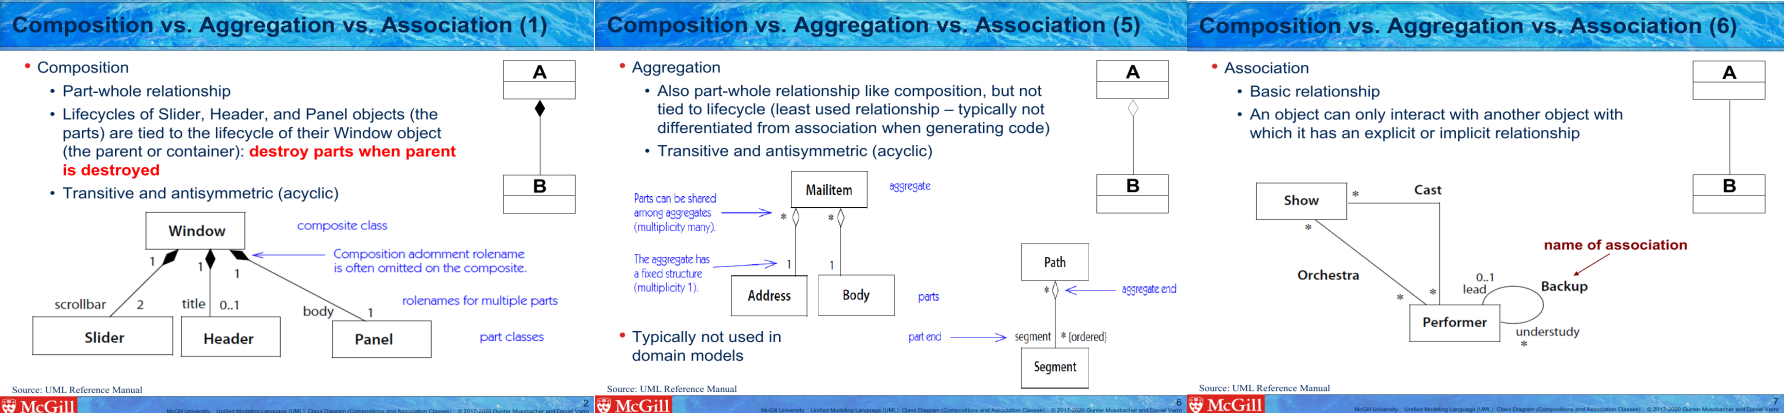
\includegraphics[width=0.9\textwidth]{images/composition_aggregation_association.png}
\end{tabular} \medskip


\noindent \textbf{Missing aggregation} \medskip

\noindent Level 1: Highlight solution \medskip

\noindent Level 2: Text response: \medskip

\begin{tabular}{|p{0.9\linewidth}}
What is the relationship between these classes?
\end{tabular} \medskip

\noindent Level 3: Parametrized response: \medskip

\begin{tabular}{|p{0.9\linewidth}}
How would you capture that a \verb|${classOne}| has a \verb|${classTwo}|?
\end{tabular} \medskip

\noindent Level 4: Resource response with Reference: \medskip

\begin{tabular}{|p{0.9\linewidth}}
Please review the _Composition vs. Aggregation vs. Association_ section of 
the \textit{UML Class Diagram lecture slides} to 
better understand these relationships and where they are used.

\\
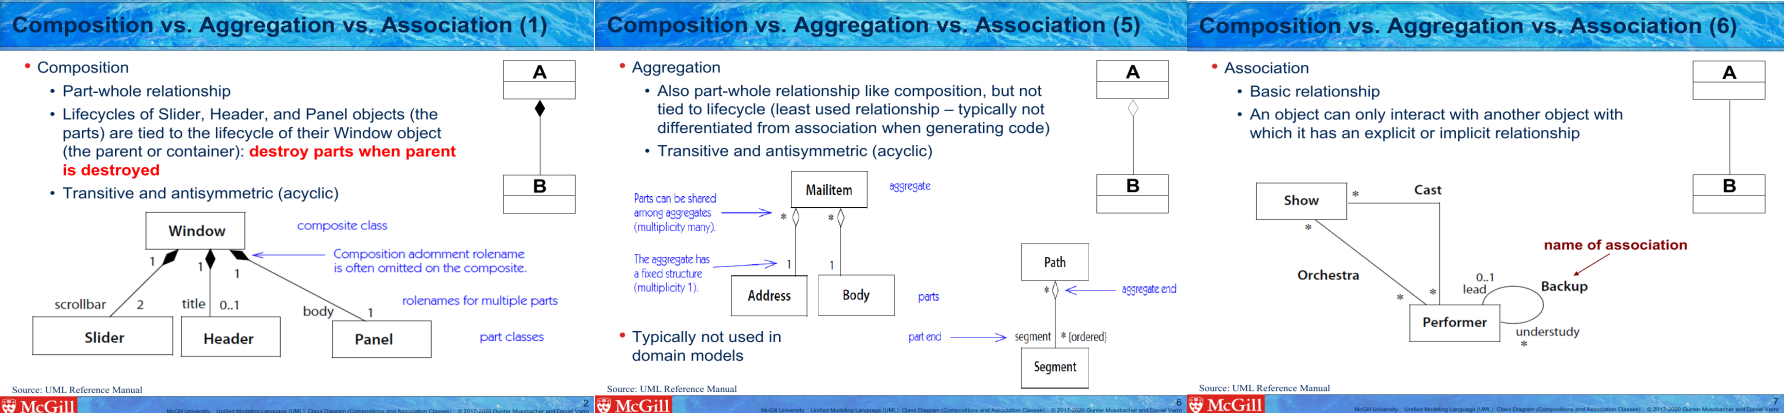
\includegraphics[width=0.9\textwidth]{images/composition_aggregation_association.png}
\end{tabular} \medskip


\noindent \textbf{Missing n-ary association} \medskip

\noindent Level 1: Highlight solution \medskip

\noindent Level 2: Text response: \medskip

\begin{tabular}{|p{0.9\linewidth}}
What is the relationship between these classes?
\end{tabular} \medskip

\noindent Level 3: Parametrized response: \medskip

\begin{tabular}{|p{0.9\linewidth}}
How would you capture the relationship between \verb|${classOne}|, \verb|${classTwo}|, [and] \verb|${classThree}|[, [and] \verb|${classFour}|[, [and] \verb|${classFive}|]]?
\end{tabular} \medskip

\noindent Level 4: Resource response with Reference: \medskip

\begin{tabular}{|p{0.9\linewidth}}
Please review the _Composition vs. Aggregation vs. Association_ section of 
the \textit{UML Class Diagram lecture slides} to 
better understand these relationships and where they are used.

\\
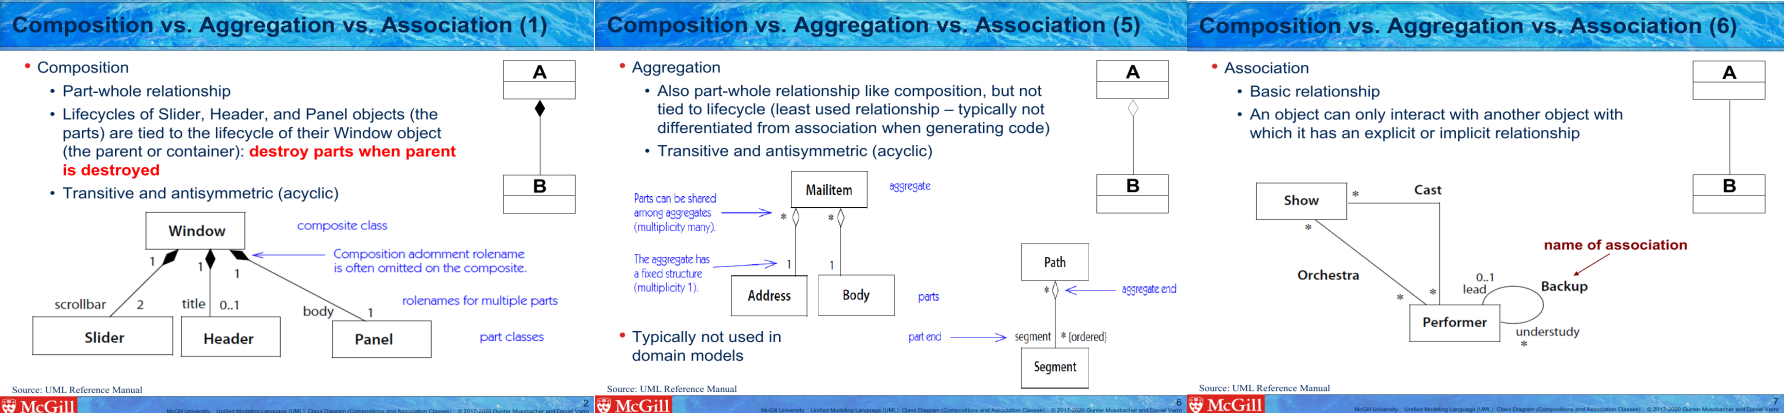
\includegraphics[width=0.9\textwidth]{images/composition_aggregation_association.png}
\end{tabular} \medskip


\noindent \textbf{Using attribute instead of association} \medskip

\noindent Level 1: Highlight solution \medskip

\noindent Level 2: Text response: \medskip

\begin{tabular}{|p{0.9\linewidth}}
Remember that attributes are simple pieces of data.
\end{tabular} \medskip

\noindent Level 3: Parametrized response: \medskip

\begin{tabular}{|p{0.9\linewidth}}
\verb|${includingClass.attributeName}| should be its own class.
\end{tabular} \medskip

\noindent Level 4: Resource response with Quiz: \medskip

\begin{tabular}{|p{0.9\linewidth}}
Pick the classes which are modeled correctly.

\begin{itemize}
    \item[$\square$] class Person \{ address; \}
    \item[$\square$] class Person \{ * Person -- 1 Address; \}; class Address \{\}
    \item[$\square$] class Loan \{ libraryPatron; \}
\end{itemize}

\end{tabular} \medskip


\subsubsection{Extra association mistakes}

\noindent \textbf{Representing an action with an association} \medskip

\noindent Level 1: Highlight solution \medskip

\noindent Level 2: Text response: \medskip

\begin{tabular}{|p{0.9\linewidth}}
Is association the best way to model this concept?
\end{tabular} \medskip

\noindent Level 3: Parametrized response: \medskip

\begin{tabular}{|p{0.9\linewidth}}
\verb|${actionName}| should not be modeled as an association.
\end{tabular} \medskip

\begin{tabular}{|p{0.9\linewidth}}
\verb|${actionName}| does not need be modeled as part of a domain model.
\end{tabular} \medskip

\noindent Level 4: Resource response with Reference: \medskip

\begin{tabular}{|p{0.9\linewidth}}
Please review the \textit{domain modeling lecture} to know which concepts should be a part of a domain model.
\end{tabular} \medskip


\noindent \textbf{Extra association} \medskip

\noindent Level 1: Highlight solution \medskip

\noindent Level 2: Text response: \medskip

\begin{tabular}{|p{0.9\linewidth}}
Is this association really necessary?
\end{tabular} \medskip

\noindent Level 3: Parametrized response: \medskip

\begin{tabular}{|p{0.9\linewidth}}
The relationship between \verb|${classOne}| and \verb|${classTwo}| is not expressed in the problem description[, but there is a similar relationship with \verb|${classThree}| that is missing].
\end{tabular} \medskip

\begin{tabular}{|p{0.9\linewidth}}
The relationship between \verb|${classOne}| and \verb|${classTwo}| is redundant since we can access \verb|${classTwo}| from \verb|${classOne}| via \verb|${classThree}|.
\end{tabular} \medskip

\noindent Level 4: Resource response with Quiz: \medskip

\begin{tabular}{|p{0.9\linewidth}}
Find all the redunandant associations in this class diagram (TODO).
\end{tabular} \medskip



\begin{tabular}{|p{0.9\linewidth}}
Write pseudocode to navigate between ClassOne and ClassTwo in this class diagram (TODO).
\end{tabular} \medskip


\noindent \textbf{Extra aggregation} \medskip

\noindent Level 1: Highlight solution \medskip

\noindent Level 2: Text response: \medskip

\begin{tabular}{|p{0.9\linewidth}}
Is this aggregation really necessary?
\end{tabular} \medskip

\noindent Level 3: Parametrized response: \medskip

\begin{tabular}{|p{0.9\linewidth}}
The relationship between \verb|${classOne}| and \verb|${classTwo}| is redundant.
\end{tabular} \medskip


\noindent \textbf{Extra n-ary association} \medskip

\noindent Level 1: Highlight solution \medskip

\noindent Level 2: Text response: \medskip

\begin{tabular}{|p{0.9\linewidth}}
Is this association really necessary?
\end{tabular} \medskip

\noindent Level 3: Parametrized response: \medskip

\begin{tabular}{|p{0.9\linewidth}}
The relationship between the highlighted classes is redundant.
\end{tabular} \medskip


\subsubsection{Association type mistakes}

\noindent \textbf{Using aggregation instead of association} \medskip

\noindent Level 1: Highlight solution \medskip

\noindent Level 2: Text response: \medskip

\begin{tabular}{|p{0.9\linewidth}}
What is the relationship between these two concepts?
\end{tabular} \medskip

\noindent Level 3: Parametrized response: \medskip

\begin{tabular}{|p{0.9\linewidth}}
The relationship between \verb|${containedClass}| and \verb|${containerClass}| can be modeled with a simple association.
\end{tabular} \medskip

\noindent Level 4: Resource response with Reference: \medskip

\begin{tabular}{|p{0.9\linewidth}}
Please review the _Composition vs. Aggregation vs. Association_ section of 
the \textit{UML Class Diagram lecture slides} to 
better understand these relationships and where they are used.

\\
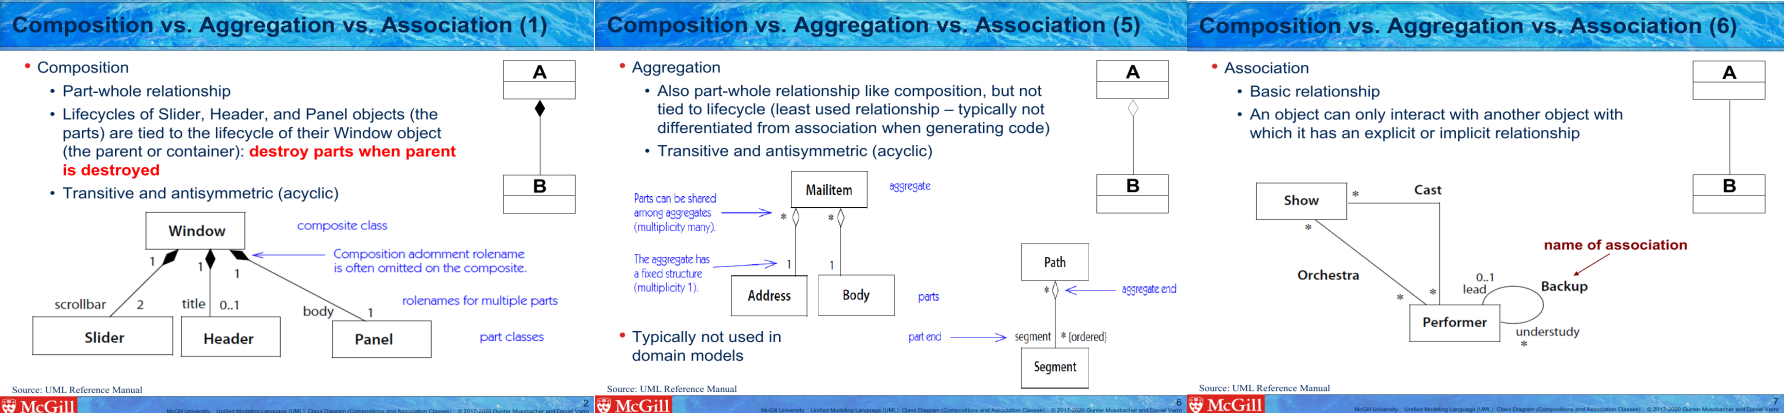
\includegraphics[width=0.9\textwidth]{images/composition_aggregation_association.png}
\end{tabular} \medskip


\noindent \textbf{Using composition instead of association} \medskip

\noindent Level 1: Highlight solution \medskip

\noindent Level 2: Text response: \medskip

\begin{tabular}{|p{0.9\linewidth}}
What is the relationship between these two concepts?
\end{tabular} \medskip

\noindent Level 3: Parametrized response: \medskip

\begin{tabular}{|p{0.9\linewidth}}
Why is \verb|${incorrectlyContainedClass}| contained in \verb|${containerClass}|?
\end{tabular} \medskip

\noindent Level 4: Resource response with Reference: \medskip

\begin{tabular}{|p{0.9\linewidth}}
Please review the _Composition vs. Aggregation vs. Association_ section of 
the \textit{UML Class Diagram lecture slides} to 
better understand these relationships and where they are used.

\\
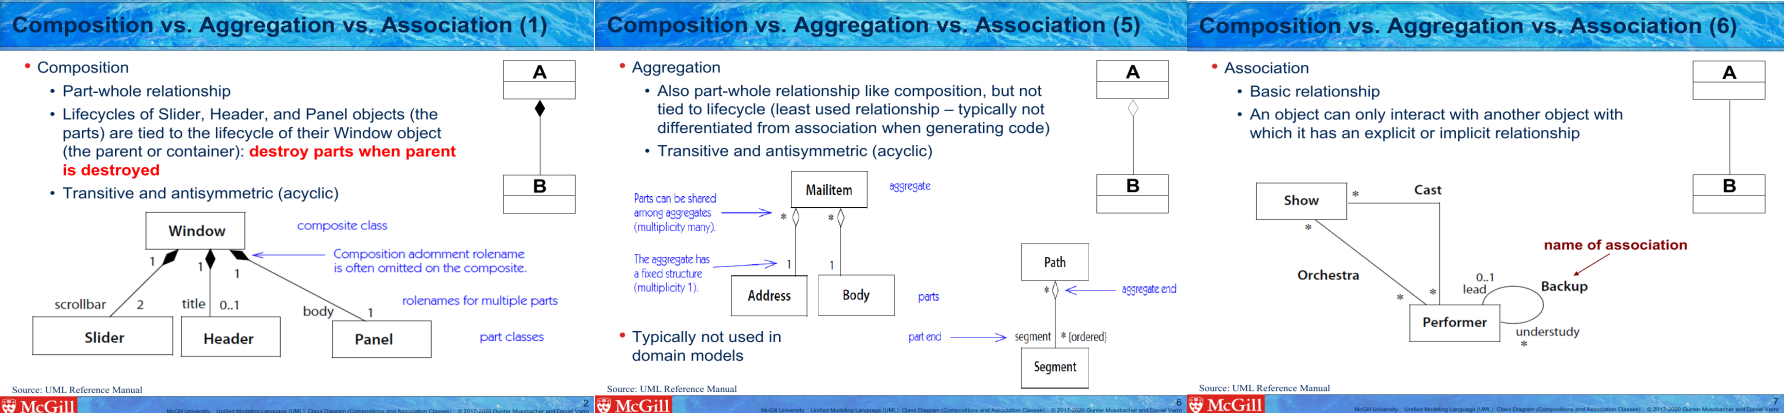
\includegraphics[width=0.9\textwidth]{images/composition_aggregation_association.png}
\end{tabular} \medskip


\noindent \textbf{Using directed association instead of undirected association} \medskip

\noindent Level 1: Highlight solution \medskip

\noindent Level 2: Text response: \medskip

\begin{tabular}{|p{0.9\linewidth}}
Is there anything special about this association?
\end{tabular} \medskip

\noindent Level 3: Parametrized response: \medskip

\begin{tabular}{|p{0.9\linewidth}}
The association between \verb|${classOne}| and \verb|${classTwo}| should be undirected[ from \verb|${classOne}| to \verb|${classTwo}|].
\end{tabular} \medskip

\noindent Level 4: 
\noindent \textbf{Using undirected association instead of directed association} \medskip

\noindent Level 1: Highlight solution \medskip

\noindent Level 2: Text response: \medskip

\begin{tabular}{|p{0.9\linewidth}}
Is there anything special about this association?
\end{tabular} \medskip

\noindent Level 3: Parametrized response: \medskip

\begin{tabular}{|p{0.9\linewidth}}
The association between \verb|${classOne}| and \verb|${classTwo}| should be directed[ from \verb|${classOne}| to \verb|${classTwo}|].
\end{tabular} \medskip

\noindent Level 4: 
\noindent \textbf{Using composition instead of aggregation} \medskip

\noindent Level 1: Highlight solution \medskip

\noindent Level 2: Text response: \medskip

\begin{tabular}{|p{0.9\linewidth}}
Is this the best relationship to use here?
\end{tabular} \medskip

\noindent Level 3: Parametrized response: \medskip

\begin{tabular}{|p{0.9\linewidth}}
The composition between \verb|${containedClass}| and \verb|${containerClass}| is better modeled using aggregation.
\end{tabular} \medskip

\noindent Level 4: Resource response with Reference: \medskip

\begin{tabular}{|p{0.9\linewidth}}
Please review the _Composition vs. Aggregation vs. Association_ section of 
the \textit{UML Class Diagram lecture slides} to 
better understand these relationships and where they are used.

\\
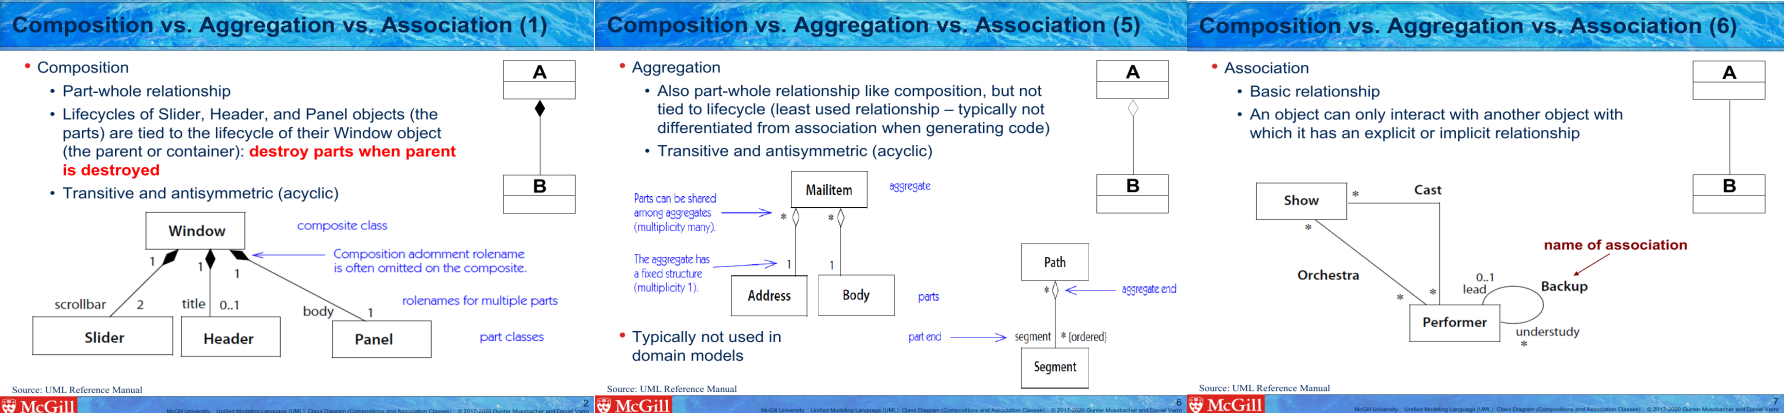
\includegraphics[width=0.9\textwidth]{images/composition_aggregation_association.png}
\end{tabular} \medskip


\noindent \textbf{Using binary association instead of n-ary association} \medskip

\noindent Level 1: Highlight solution \medskip

\noindent Level 2: Text response: \medskip

\begin{tabular}{|p{0.9\linewidth}}
Can you model this relationship more precisely?
\end{tabular} \medskip

\noindent Level 3: Parametrized response: \medskip

\begin{tabular}{|p{0.9\linewidth}}
Use a \verb|${n}|-ary association to represent this relationship.
\end{tabular} \medskip

\noindent Level 4: Resource response with Reference: \medskip

\begin{tabular}{|p{0.9\linewidth}}
Please review the \textit{Association} part of the Class Diagram lecture.
\end{tabular} \medskip


\noindent \textbf{Using n-ary association instead of binary association} \medskip

\noindent Level 1: Highlight solution \medskip

\noindent Level 2: Text response: \medskip

\begin{tabular}{|p{0.9\linewidth}}
Can you model this relationship more precisely?
\end{tabular} \medskip

\noindent Level 3: Text response: \medskip

\begin{tabular}{|p{0.9\linewidth}}
Use a binary association to represent this relationship.
\end{tabular} \medskip

\noindent Level 4: Resource response with Reference: \medskip

\begin{tabular}{|p{0.9\linewidth}}
Please review the \textit{Association} part of the Class Diagram lecture.
\end{tabular} \medskip


\noindent \textbf{Using intermediate class instead of n-ary association} \medskip

\noindent Level 1: Highlight solution \medskip

\noindent Level 2: Text response: \medskip

\begin{tabular}{|p{0.9\linewidth}}
Can you model this relationship in a different way?
\end{tabular} \medskip

\noindent Level 3: Parametrized response: \medskip

\begin{tabular}{|p{0.9\linewidth}}
Use a \verb|${n}|-ary association to represent this relationship.
\end{tabular} \medskip

\noindent Level 4: Resource response with Reference: \medskip

\begin{tabular}{|p{0.9\linewidth}}
Please review the \textit{Association} part of the Class Diagram lecture.
\end{tabular} \medskip


\subsubsection{Association name mistakes}

\noindent \textbf{Missing association name when one was expected} \medskip

\noindent Level 1: Highlight solution \medskip

\noindent Level 2: Text response: \medskip

\begin{tabular}{|p{0.9\linewidth}}
Something is missing here.
\end{tabular} \medskip

\noindent Level 3: Parametrized response: \medskip

\begin{tabular}{|p{0.9\linewidth}}
Can you give this association a name?
\end{tabular} \medskip

\noindent Level 4: Parametrized response: \medskip

\begin{tabular}{|p{0.9\linewidth}}
This association should be named \verb|${associationName}|.
\end{tabular} \medskip

\noindent Level 5: Resource response with Reference: \medskip

\begin{tabular}{|p{0.9\linewidth}}
Please review the \textit{Association} and \textit{Noun Analysis} parts of the Class Diagram lecture.
\end{tabular} \medskip


\noindent \textbf{Bad association name spelling} \medskip

\noindent Level 1: Highlight solution \medskip

\noindent Level 2: Text response: \medskip

\begin{tabular}{|p{0.9\linewidth}}
Check your spelling here.
\end{tabular} \medskip

\noindent Level 3: Parametrized response: \medskip

\begin{tabular}{|p{0.9\linewidth}}
\verb|${associationName}| is misspelled.[ Use the same spelling as the problem description.]
\end{tabular} \medskip

\noindent Level 4: Resource response with Reference: \medskip

\begin{tabular}{|p{0.9\linewidth}}
Please review the \textit{Association} and \textit{Noun Analysis} parts of the Class Diagram lecture.
\end{tabular} \medskip


\noindent \textbf{Similar association name} \medskip

\noindent Level 1: Highlight solution \medskip

\noindent Level 2: Text response: \medskip

\begin{tabular}{|p{0.9\linewidth}}
Can you double check this association name?
\end{tabular} \medskip

\noindent Level 3: Parametrized response: \medskip

\begin{tabular}{|p{0.9\linewidth}}
The \verb|${similarYetIncorrectAssociationName}| association has a name that is not quite right.
\end{tabular} \medskip

\noindent Level 4: Parametrized response: \medskip

\begin{tabular}{|p{0.9\linewidth}}
The \verb|${similarYetIncorrectAssociationName}| association should be changed to \verb|${correctAssociationName}|.
\end{tabular} \medskip

\noindent Level 5: Resource response with Reference: \medskip

\begin{tabular}{|p{0.9\linewidth}}
Please review the \textit{Association} and \textit{Noun Analysis} parts of the Class Diagram lecture.
\end{tabular} \medskip


\subsubsection{Multiplicity mistakes}

\noindent \textbf{Infinite recursive dependency} \medskip

\noindent Level 1: Highlight solution \medskip

\noindent Level 2: Text response: \medskip

\begin{tabular}{|p{0.9\linewidth}}
Can you double check (this$|$these) association(s)?
\end{tabular} \medskip

\noindent Level 3: Text response: \medskip

\begin{tabular}{|p{0.9\linewidth}}
The multiplicities for this(ese) association(s) are incorrect.
\end{tabular} \medskip

\noindent Level 4: Parametrized response: \medskip

\begin{tabular}{|p{0.9\linewidth}}
Does every \verb|${class1}| have exactly \verb|${wrongMultiplicity}| \verb|${rolename}|[s]?
\end{tabular} \medskip

\begin{tabular}{|p{0.9\linewidth}}
How many \verb|${class1}|'s does a \verb|${class2}| have?
\end{tabular} \medskip

\begin{tabular}{|p{0.9\linewidth}}
Double check the multiplicites between \verb|${class1}|, \verb|${class2}|, and \verb|${class3}|.
\end{tabular} \medskip

\noindent Level 5: Resource response with Quiz: \medskip

\begin{tabular}{|p{0.9\linewidth}}
Edit the class diagram to allow creating a `Foo`
\end{tabular} \medskip


\noindent \textbf{Wrong multiplicity} \medskip

\noindent Level 1: Highlight solution \medskip

\noindent Level 2: Text response: \medskip

\begin{tabular}{|p{0.9\linewidth}}
Can you double check this association?
\end{tabular} \medskip

\noindent Level 3: Text response: \medskip

\begin{tabular}{|p{0.9\linewidth}}
The multiplicit(y$|$ies) for this association (is$|$are) incorrect.
\end{tabular} \medskip

\noindent Level 4: Parametrized response: \medskip

\begin{tabular}{|p{0.9\linewidth}}
How many \verb|${class1}|'s does a \verb|${class2}| have? [And how many \verb|${class2}|'s does \verb|${class1}| have?]
\end{tabular} \medskip

\noindent Level 5: Resource response with Quiz: \medskip

\begin{tabular}{|p{0.9\linewidth}}
Pick the associations with correct multiplicities

\begin{itemize}
    \item[$\square$] 1 EmployeeRole -- 1 Person;
    \item[$\square$] * Episode -- 1 TvSeries;
    \item[$\square$] * Bank -- 1 Client;
\end{itemize}

\end{tabular} \medskip


\noindent \textbf{Missing multiplicity} \medskip

\noindent Level 1: Highlight solution \medskip

\noindent Level 2: Text response: \medskip

\begin{tabular}{|p{0.9\linewidth}}
Can you double check this association?
\end{tabular} \medskip

\noindent Level 3: Text response: \medskip

\begin{tabular}{|p{0.9\linewidth}}
The multiplicit(y$|$ies) for this association (is$|$are) missing.
\end{tabular} \medskip

\noindent Level 4: Parametrized response: \medskip

\begin{tabular}{|p{0.9\linewidth}}
How many \verb|${class1}|'s does a \verb|${class2}| have? [And how many \verb|${class2}|'s does \verb|${class1}| have?]
\end{tabular} \medskip

\noindent Level 5: Resource response with Quiz: \medskip

\begin{tabular}{|p{0.9\linewidth}}
Pick the associations with correct multiplicities

\begin{itemize}
    \item[$\square$] 1 EmployeeRole -- 1 Person;
    \item[$\square$] * Episode -- 1 TvSeries;
    \item[$\square$] * Bank -- 1 Client;
\end{itemize}

\end{tabular} \medskip


\subsubsection{Role name mistakes}

\noindent \textbf{Missing role names} \medskip

\noindent Level 1: Highlight solution \medskip

\noindent Level 2: Text response: \medskip

\begin{tabular}{|p{0.9\linewidth}}
Can you model this relationship more precisely?
\end{tabular} \medskip

\noindent Level 3: Text response: \medskip

\begin{tabular}{|p{0.9\linewidth}}
The multiplicities for this association are correct, but something else is missing!
\end{tabular} \medskip

\noindent Level 4: Resource response with Reference: \medskip

\begin{tabular}{|p{0.9\linewidth}}
Can you think of appropriate \textit{role names}
for this association? Role names help identify the role a class plays in a
relationship and can be important if there is more than one relationship
between the same two classes.

\\
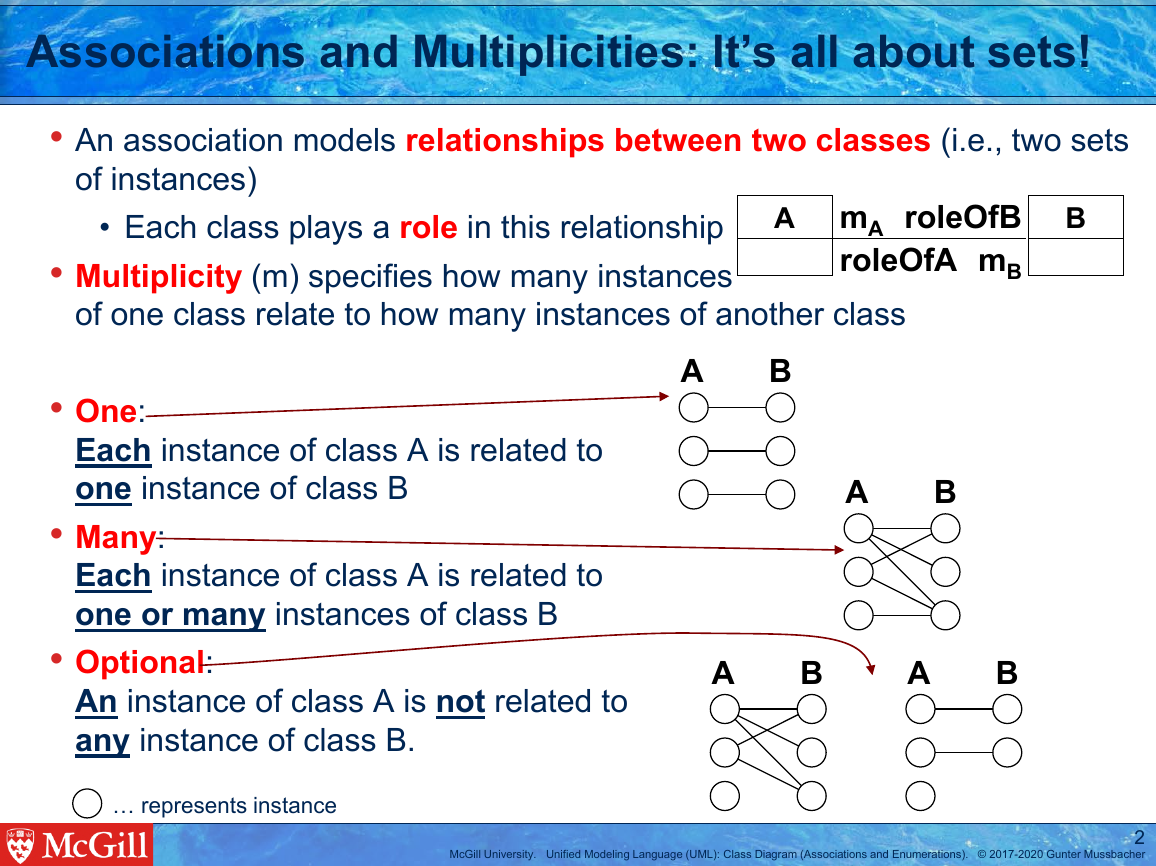
\includegraphics[width=0.6\textwidth]{images/role_name.png}

\end{tabular} \medskip


\noindent \textbf{Role should be static} \medskip

\noindent Level 1: Highlight solution \medskip

\noindent Level 2: Text response: \medskip

\begin{tabular}{|p{0.9\linewidth}}
Isn't there something special about this role name?
\end{tabular} \medskip

\noindent Level 3: Parametrized response: \medskip

\begin{tabular}{|p{0.9\linewidth}}
\verb|${roleName}| should be static, because it applies to all instances of the association between \verb|${class1}| and \verb|${class2}|.
\end{tabular} \medskip

\noindent Level 4: Resource response with Reference: \medskip

\begin{tabular}{|p{0.9\linewidth}}
Please review the \textit{Association} part of the Class Diagram lecture.
\end{tabular} \medskip


\noindent \textbf{Role should not be static} \medskip

\noindent Level 1: Highlight solution \medskip

\noindent Level 2: Text response: \medskip

\begin{tabular}{|p{0.9\linewidth}}
Isn't there something special about this role name?
\end{tabular} \medskip

\noindent Level 3: Parametrized response: \medskip

\begin{tabular}{|p{0.9\linewidth}}
\verb|${roleName}| should not be static, because it doesn't apply to all instances of the association between \verb|${class1}| and \verb|${class2}|.
\end{tabular} \medskip

\noindent Level 4: Resource response with Reference: \medskip

\begin{tabular}{|p{0.9\linewidth}}
Please review the \textit{Association} part of the Class Diagram lecture.
\end{tabular} \medskip


\noindent \textbf{Bad role name spelling} \medskip

\noindent Level 1: Highlight solution \medskip

\noindent Level 2: Text response: \medskip

\begin{tabular}{|p{0.9\linewidth}}
Check your spelling here.
\end{tabular} \medskip

\noindent Level 3: Parametrized response: \medskip

\begin{tabular}{|p{0.9\linewidth}}
\verb|${roleName}| is misspelled.[ Use the same spelling as the problem description.]
\end{tabular} \medskip

\noindent Level 4: Resource response with Reference: \medskip

\begin{tabular}{|p{0.9\linewidth}}
Please review the \textit{Association} and \textit{Noun Analysis} parts of the Class Diagram lecture.
\end{tabular} \medskip


\noindent \textbf{Similar role name} \medskip

\noindent Level 1: Highlight solution \medskip

\noindent Level 2: Text response: \medskip

\begin{tabular}{|p{0.9\linewidth}}
Can you double check this role name?
\end{tabular} \medskip

\noindent Level 3: Parametrized response: \medskip

\begin{tabular}{|p{0.9\linewidth}}
The \verb|${wrongRoleName}| role name is not quite right.
\end{tabular} \medskip

\noindent Level 4: Parametrized response: \medskip

\begin{tabular}{|p{0.9\linewidth}}
The \verb|${wrongRoleName}| role name should be changed to \verb|${correctRoleName}|.
\end{tabular} \medskip

\noindent Level 5: Resource response with Reference: \medskip

\begin{tabular}{|p{0.9\linewidth}}
Can you think of appropriate \textit{role names}
for this association? Role names help identify the role a class plays in a
relationship and can be important if there is more than one relationship
between the same two classes.

\\
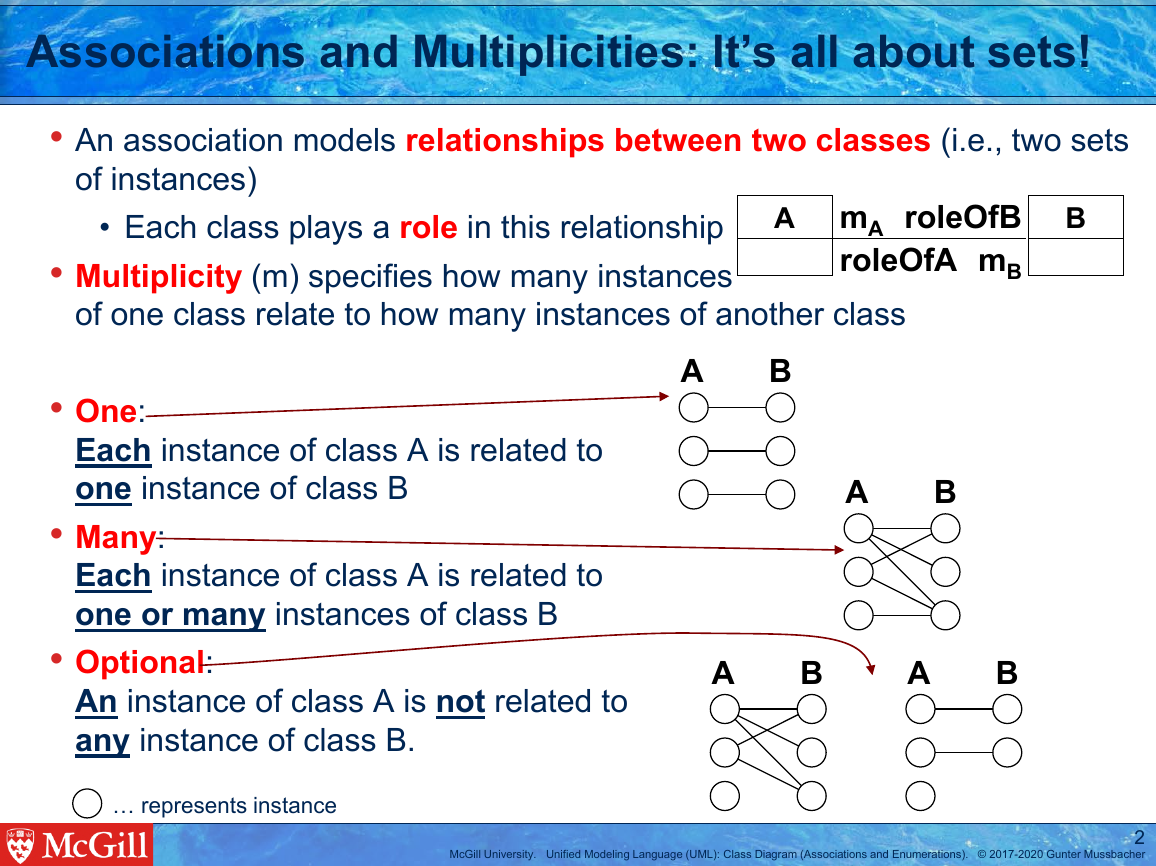
\includegraphics[width=0.6\textwidth]{images/role_name.png}

\end{tabular} \medskip


\noindent \textbf{Wrong role name but correct association} \medskip

\noindent Level 1: Highlight solution \medskip

\noindent Level 2: Text response: \medskip

\begin{tabular}{|p{0.9\linewidth}}
Can you double check this role name?
\end{tabular} \medskip

\noindent Level 3: Parametrized response: \medskip

\begin{tabular}{|p{0.9\linewidth}}
The \verb|${wrongRoleName}| role name is not correct.
\end{tabular} \medskip

\noindent Level 4: Parametrized response: \medskip

\begin{tabular}{|p{0.9\linewidth}}
The \verb|${wrongRoleName}| role name should be changed to \verb|${correctRoleName}|.
\end{tabular} \medskip

\noindent Level 5: Resource response with Reference: \medskip

\begin{tabular}{|p{0.9\linewidth}}
Can you think of appropriate \textit{role names}
for this association? Role names help identify the role a class plays in a
relationship and can be important if there is more than one relationship
between the same two classes.

\\
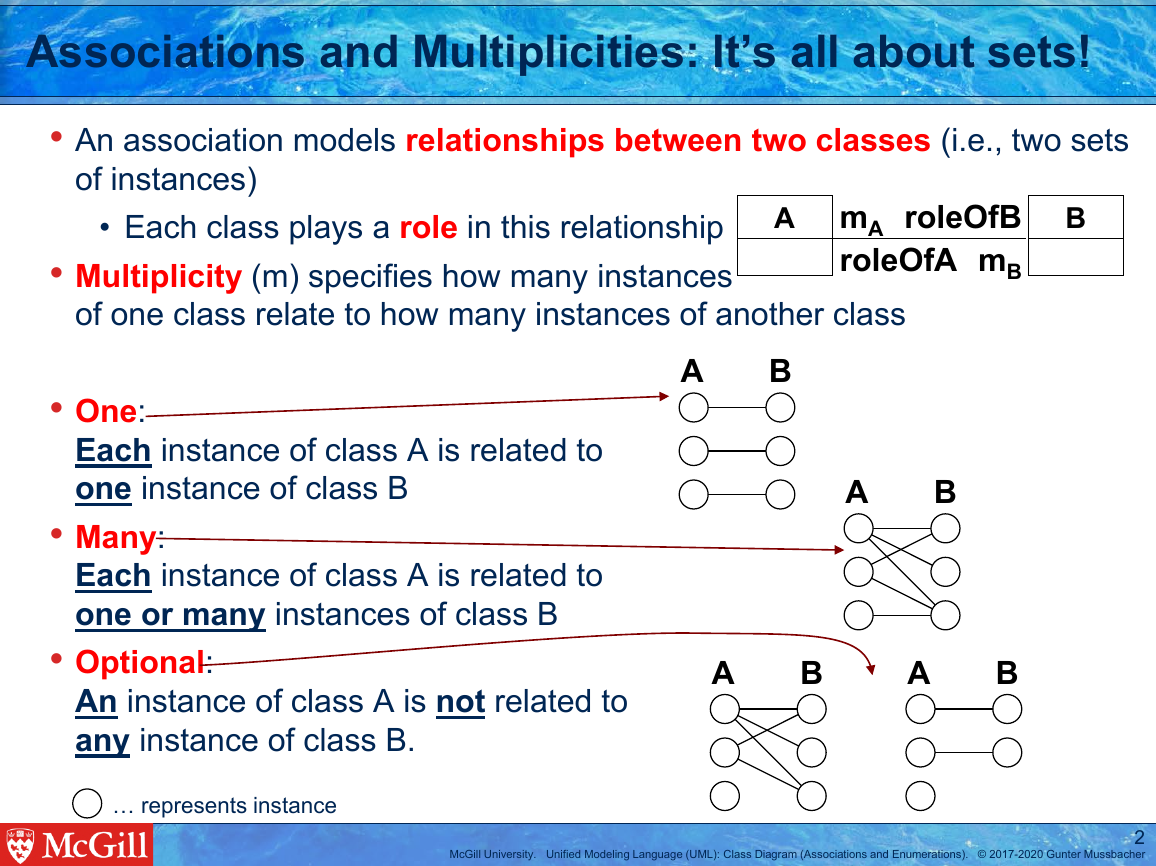
\includegraphics[width=0.6\textwidth]{images/role_name.png}

\end{tabular} \medskip


\subsubsection{Association class mistakes}

\noindent \textbf{Missing association class} \medskip

\noindent Level 1: Highlight solution \medskip

\noindent Level 2: Text response: \medskip

\begin{tabular}{|p{0.9\linewidth}}
Can you model this relationship more precisely?
\end{tabular} \medskip

\noindent Level 3: Parametrized response: \medskip

\begin{tabular}{|p{0.9\linewidth}}
Does it make sense to have multiple instances of the \verb|${inBetweenClass}| linking \verb|${firstClass}| and \verb|${secondClass}|?
\end{tabular} \medskip

\noindent Level 4: Parametrized response: \medskip

\begin{tabular}{|p{0.9\linewidth}}
The association between \verb|${firstClass}| and \verb|${secondClass}| should be modeled with an association class.
\end{tabular} \medskip

\noindent Level 5: Resource response with Reference: \medskip

\begin{tabular}{|p{0.9\linewidth}}
Association class

\\
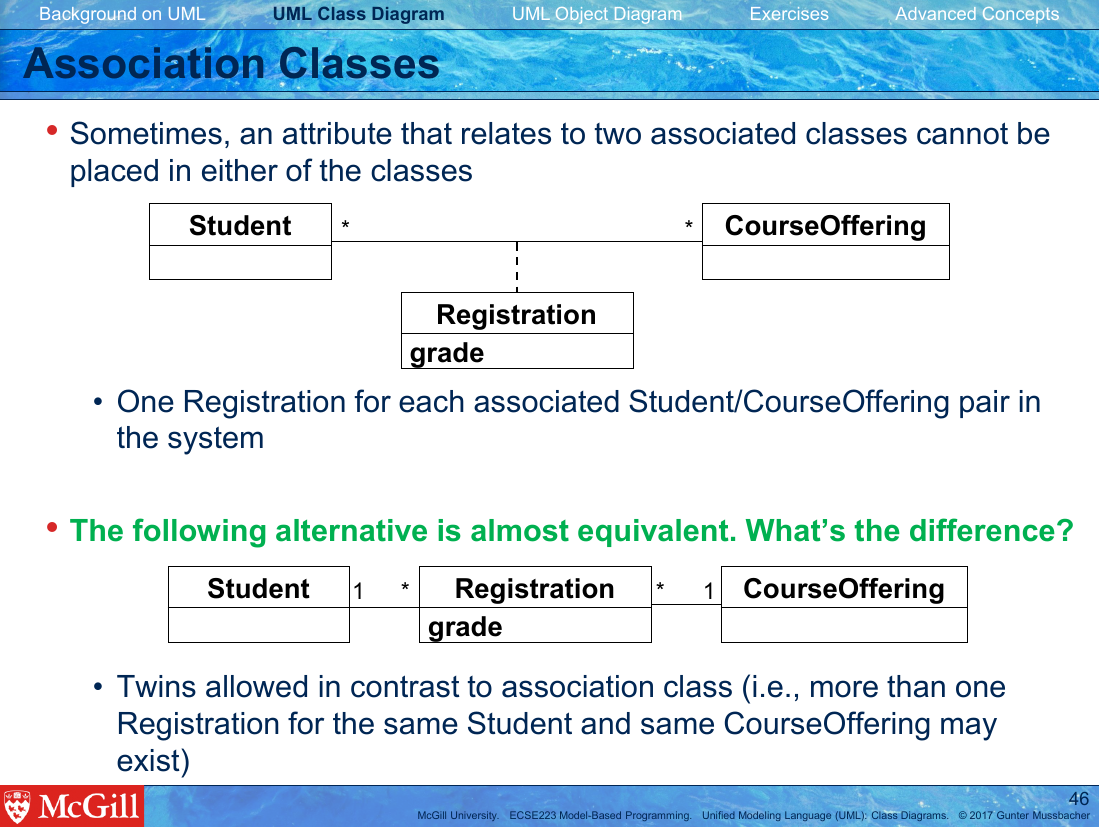
\includegraphics[width=0.6\textwidth]{images/association_class.png}
\end{tabular} \medskip


\noindent \textbf{Extra association class} \medskip

\noindent Level 1: Highlight solution \medskip

\noindent Level 2: Text response: \medskip

\begin{tabular}{|p{0.9\linewidth}}
Can you model this relationship in another way?
\end{tabular} \medskip

\noindent Level 3: Text response: \medskip

\begin{tabular}{|p{0.9\linewidth}}
Is using an association class the best way to model this?
\end{tabular} \medskip

\noindent Level 4: Parametrized response: \medskip

\begin{tabular}{|p{0.9\linewidth}}
Does it make sense to disallow multiple instances of the \verb|${inBetweenClass}| linking \verb|${firstClass}| and \verb|${secondClass}|?
\end{tabular} \medskip

\noindent Level 5: Parametrized response: \medskip

\begin{tabular}{|p{0.9\linewidth}}
The association between \verb|${firstClass}| and \verb|${secondClass}| should not be modeled with an association class.
\end{tabular} \medskip

\noindent Level 6: Resource response with Reference: \medskip

\begin{tabular}{|p{0.9\linewidth}}
Association class

\\
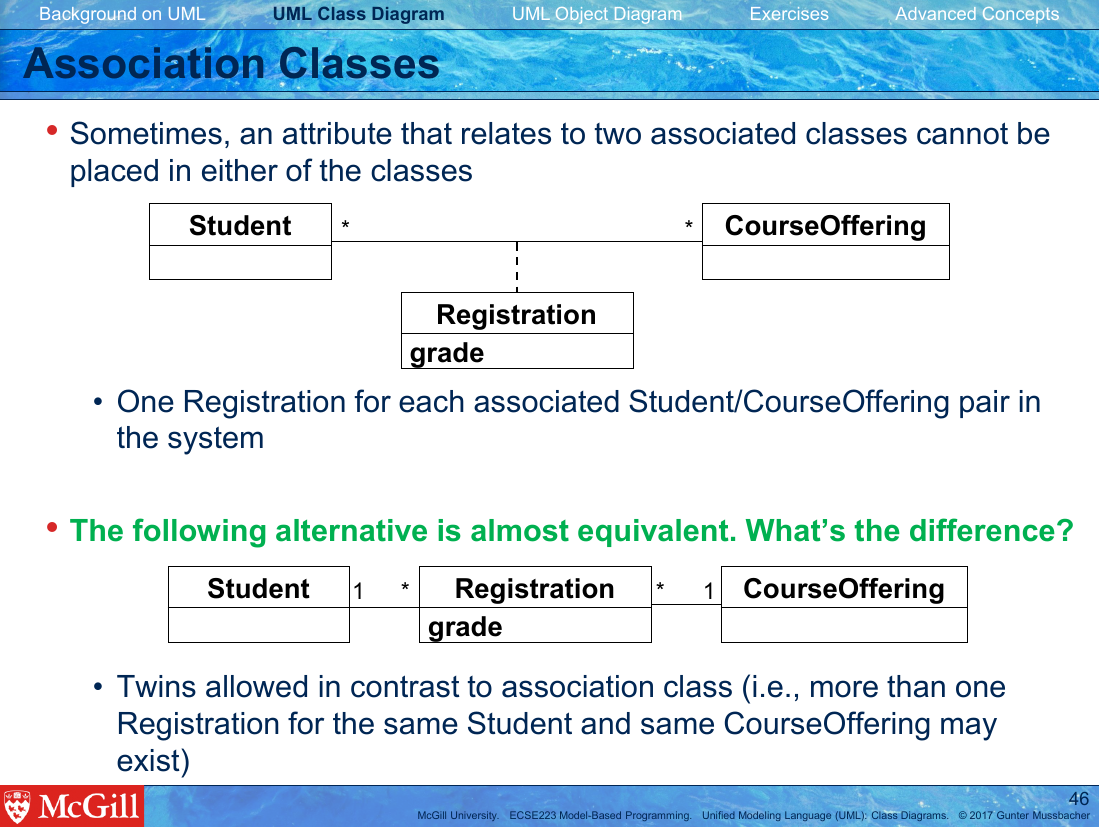
\includegraphics[width=0.6\textwidth]{images/association_class.png}
\end{tabular} \medskip


\noindent \textbf{Bad association class name spelling} \medskip

\noindent Level 1: Highlight solution \medskip

\noindent Level 2: Text response: \medskip

\begin{tabular}{|p{0.9\linewidth}}
Can you double check this class name?
\end{tabular} \medskip

\noindent Level 3: Parametrized response: \medskip

\begin{tabular}{|p{0.9\linewidth}}
The \verb|${incorrectlySpelledClassName}| class has a misspelled name.
\end{tabular} \medskip

\noindent Level 4: Parametrized response: \medskip

\begin{tabular}{|p{0.9\linewidth}}
The \verb|${incorrectlySpelledClassName}| class should be changed to \verb|${correctClassName}|.
\end{tabular} \medskip


\noindent \textbf{Association class should be regular class} \medskip

\noindent Level 1: Highlight solution \medskip

\noindent Level 2: Text response: \medskip

\begin{tabular}{|p{0.9\linewidth}}
Can you model this relationship in another way?
\end{tabular} \medskip

\noindent Level 3: Text response: \medskip

\begin{tabular}{|p{0.9\linewidth}}
Is using an association class the best way to model this?
\end{tabular} \medskip

\noindent Level 4: Parametrized response: \medskip

\begin{tabular}{|p{0.9\linewidth}}
The \verb|${assocClass}| class should be a regular class.
\end{tabular} \medskip

\noindent Level 5: Resource response with Reference: \medskip

\begin{tabular}{|p{0.9\linewidth}}
Association class

\\
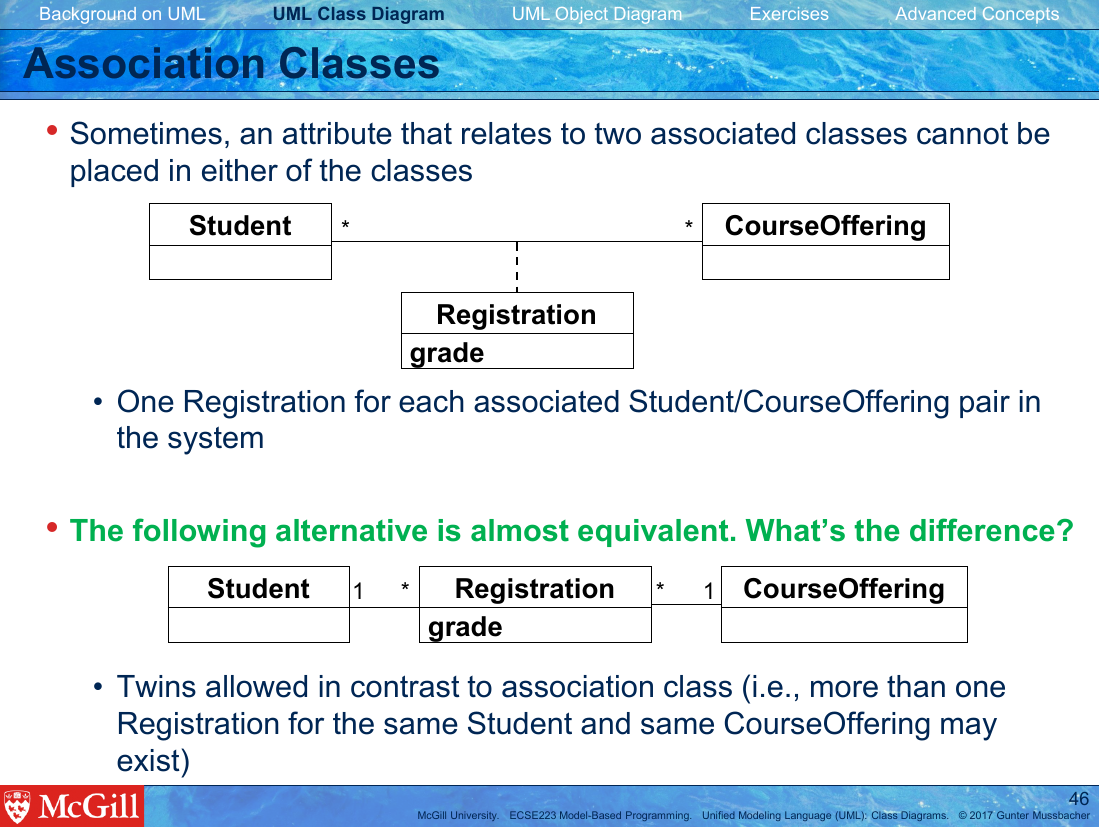
\includegraphics[width=0.6\textwidth]{images/association_class.png}
\end{tabular} \medskip


\noindent \textbf{Regular class should be association class} \medskip

\noindent Level 1: Highlight solution \medskip

\noindent Level 2: Text response: \medskip

\begin{tabular}{|p{0.9\linewidth}}
Can you model this relationship in another way?
\end{tabular} \medskip

\noindent Level 3: Text response: \medskip

\begin{tabular}{|p{0.9\linewidth}}
Is using a regular class the best way to model this?
\end{tabular} \medskip

\noindent Level 4: Parametrized response: \medskip

\begin{tabular}{|p{0.9\linewidth}}
The \verb|${assocClass}| class should be an association class.
\end{tabular} \medskip

\noindent Level 5: Resource response with Reference: \medskip

\begin{tabular}{|p{0.9\linewidth}}
Association class

\\
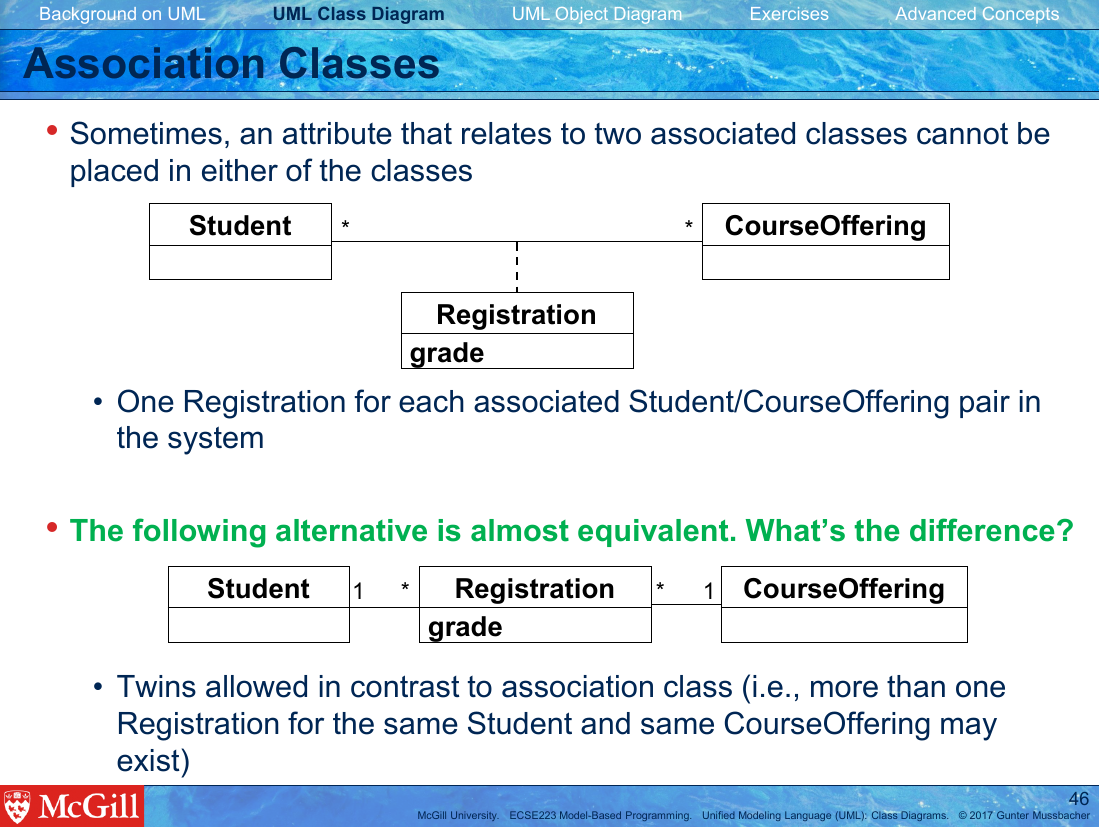
\includegraphics[width=0.6\textwidth]{images/association_class.png}
\end{tabular} \medskip


\noindent \textbf{Similar association class name} \medskip

\noindent Level 1: Highlight solution \medskip

\noindent Level 2: Text response: \medskip

\begin{tabular}{|p{0.9\linewidth}}
Can you double check this class name?
\end{tabular} \medskip

\noindent Level 3: Parametrized response: \medskip

\begin{tabular}{|p{0.9\linewidth}}
The \verb|${incorrectlySpelledClassName}| class has a name that is not quite right.
\end{tabular} \medskip

\noindent Level 4: Parametrized response: \medskip

\begin{tabular}{|p{0.9\linewidth}}
The \verb|${incorrectlySpelledClassName}| class should be changed to \verb|${correctClassName}|.
\end{tabular} \medskip



\subsection{Composition mistakes}

\subsubsection{Missing composition}

\noindent Level 1: Highlight solution \medskip

\noindent Level 2: Text response: \medskip

\begin{tabular}{|p{0.9\linewidth}}
What is the relationship between these classes?
\end{tabular} \medskip

\noindent Level 3: Parametrized response: \medskip

\begin{tabular}{|p{0.9\linewidth}}
How would you capture that a \verb|${containerClass}| contains a \verb|${containedClass}|?
\end{tabular} \medskip

\noindent Level 4: Resource response with Reference: \medskip

\begin{tabular}{|p{0.9\linewidth}}
Please review the _Composition vs. Aggregation vs. Association_ section of 
the \textit{UML Class Diagram lecture slides} to 
better understand these relationships and where they are used.

\\
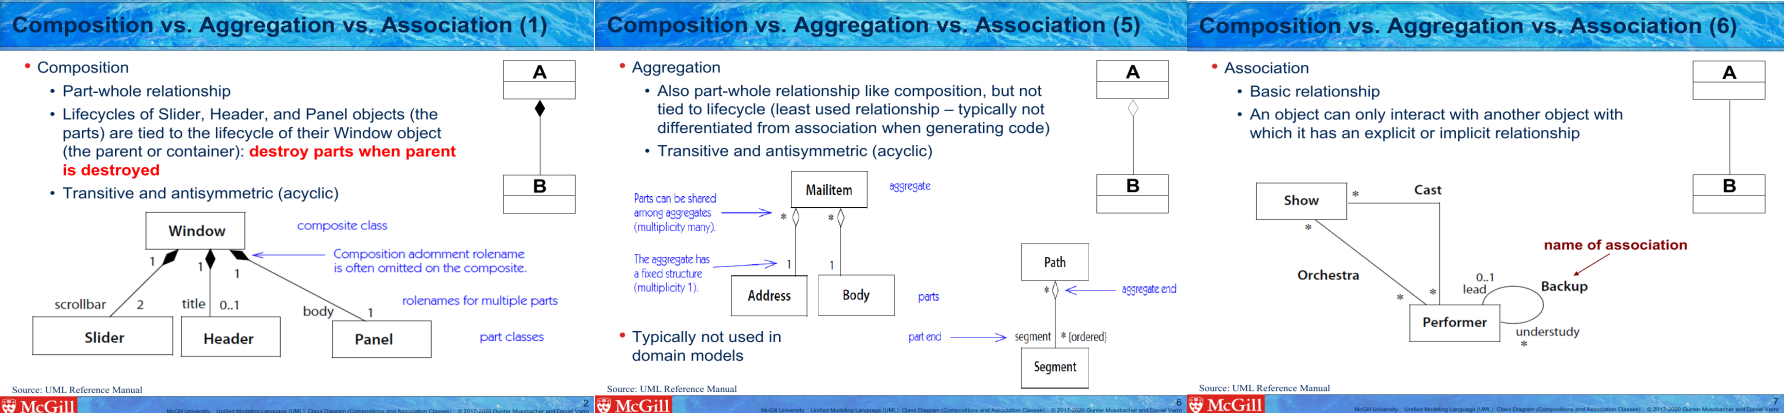
\includegraphics[width=0.9\textwidth]{images/composition_aggregation_association.png}
\end{tabular} \medskip


\subsubsection{Extra composition}

\noindent Level 1: Highlight solution \medskip

\noindent Level 2: Text response: \medskip

\begin{tabular}{|p{0.9\linewidth}}
Is this composition really necessary?
\end{tabular} \medskip

\noindent Level 3: Parametrized response: \medskip

\begin{tabular}{|p{0.9\linewidth}}
The relationship between \verb|${classOne}| and \verb|${classTwo}| is not expressed in the problem description[, but there is a similar relationship with \verb|${classThree}| that is missing].
\end{tabular} \medskip

\noindent Level 4: Resource response with Reference: \medskip

\begin{tabular}{|p{0.9\linewidth}}
Please review the _Composition vs. Aggregation vs. Association_ section of 
the \textit{UML Class Diagram lecture slides} to 
better understand these relationships and where they are used.

\\
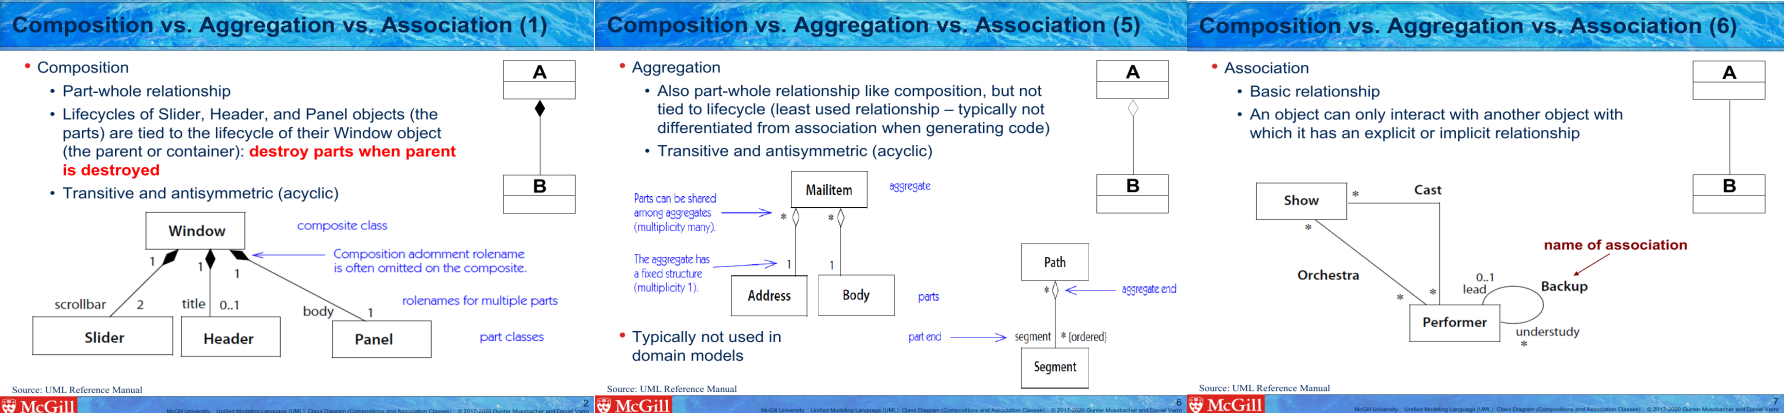
\includegraphics[width=0.9\textwidth]{images/composition_aggregation_association.png}
\end{tabular} \medskip


\subsubsection{Using association instead of aggregation}

\noindent Level 1: Highlight solution \medskip

\noindent Level 2: Text response: \medskip

\begin{tabular}{|p{0.9\linewidth}}
What is the relationship between these two concepts?
\end{tabular} \medskip

\noindent Level 3: Parametrized response: \medskip

\begin{tabular}{|p{0.9\linewidth}}
The relationship between \verb|${containedClass}| and \verb|${containerClass}| can be modeled more precisely than with a simple association.
\end{tabular} \medskip

\noindent Level 4: Resource response with Reference: \medskip

\begin{tabular}{|p{0.9\linewidth}}
Please review the _Composition vs. Aggregation vs. Association_ section of 
the \textit{UML Class Diagram lecture slides} to 
better understand these relationships and where they are used.

\\
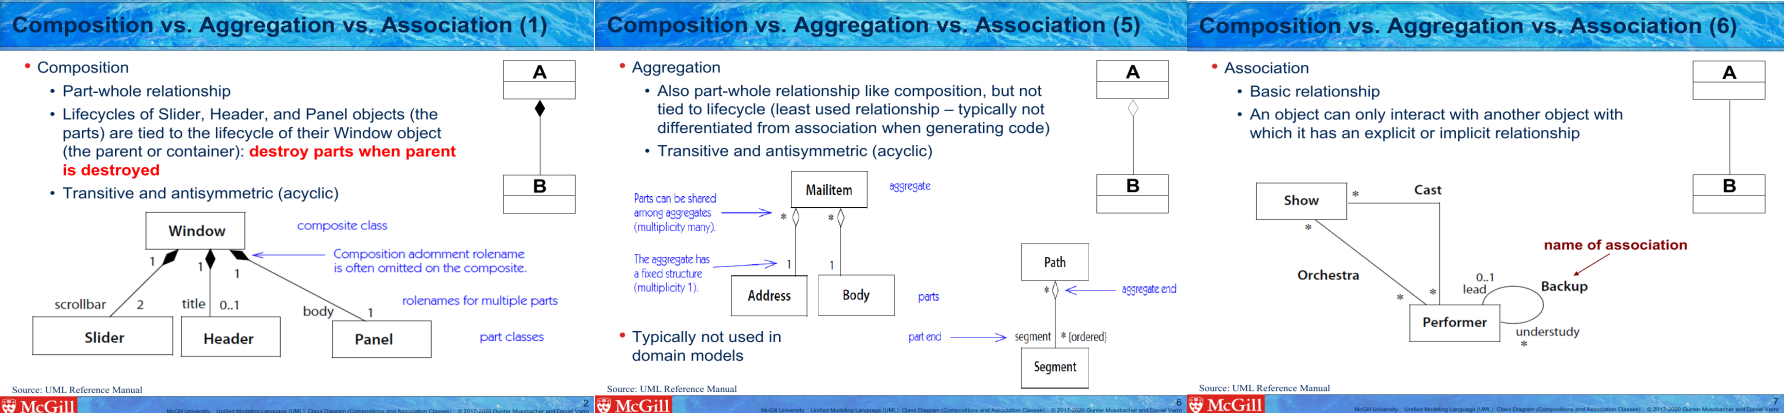
\includegraphics[width=0.9\textwidth]{images/composition_aggregation_association.png}
\end{tabular} \medskip


\subsubsection{Using association instead of composition}

\noindent Level 1: Highlight solution \medskip

\noindent Level 2: Text response: \medskip

\begin{tabular}{|p{0.9\linewidth}}
What is the relationship between these two concepts?
\end{tabular} \medskip

\noindent Level 3: Parametrized response: \medskip

\begin{tabular}{|p{0.9\linewidth}}
The relationship between \verb|${containedClass}| and \verb|${containerClass}| is more than a simple association.
\end{tabular} \medskip

\noindent Level 4: Resource response with Reference: \medskip

\begin{tabular}{|p{0.9\linewidth}}
Please review the _Composition vs. Aggregation vs. Association_ section of 
the \textit{UML Class Diagram lecture slides} to 
better understand these relationships and where they are used.

\\
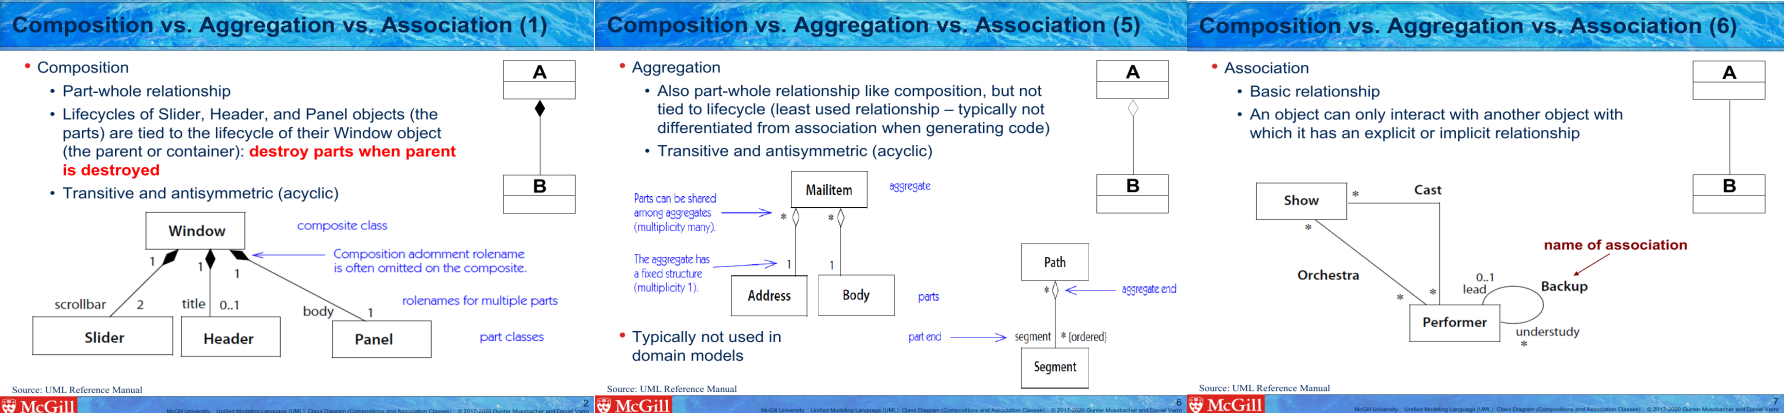
\includegraphics[width=0.9\textwidth]{images/composition_aggregation_association.png}
\end{tabular} \medskip


\subsubsection{Using aggregation instead of composition}

\noindent Level 1: Highlight solution \medskip

\noindent Level 2: Text response: \medskip

\begin{tabular}{|p{0.9\linewidth}}
Is this the best relationship to use here?
\end{tabular} \medskip

\noindent Level 3: Parametrized response: \medskip

\begin{tabular}{|p{0.9\linewidth}}
The relationship between \verb|${containedClass}| and \verb|${containerClass}| is stronger than an aggregation.
\end{tabular} \medskip

\noindent Level 4: Resource response with Reference: \medskip

\begin{tabular}{|p{0.9\linewidth}}
Please review the _Composition vs. Aggregation vs. Association_ section of 
the \textit{UML Class Diagram lecture slides} to 
better understand these relationships and where they are used.

\\
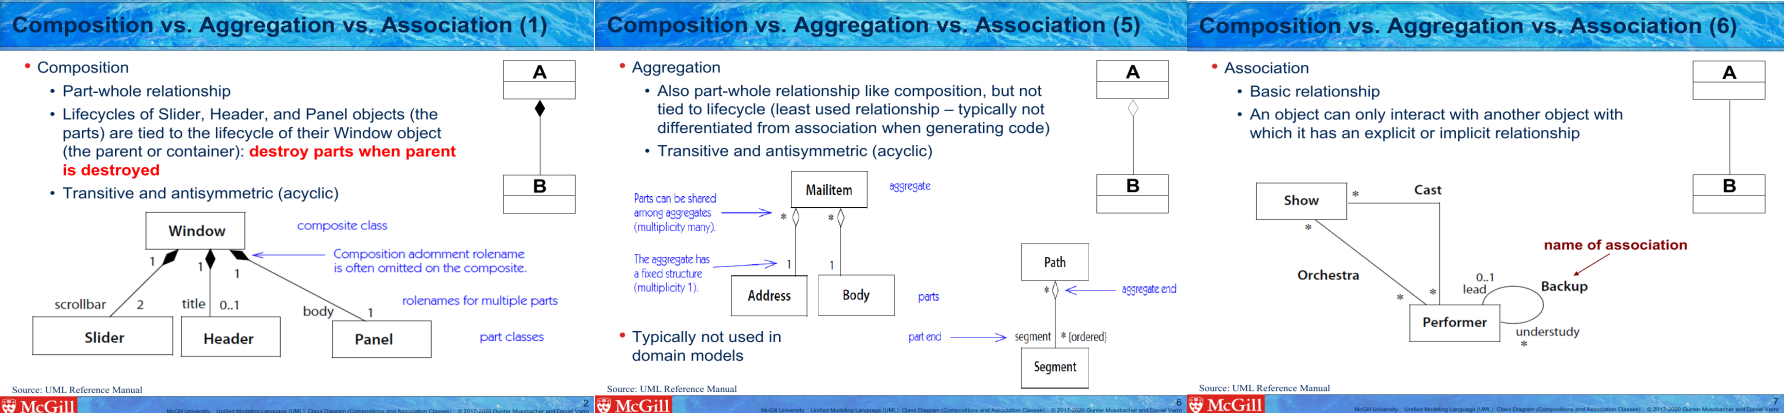
\includegraphics[width=0.9\textwidth]{images/composition_aggregation_association.png}
\end{tabular} \medskip


\subsubsection{Composed part contained in more than one parent}

\noindent Level 1: Highlight solution \medskip

\noindent Level 2: Text response: \medskip

\begin{tabular}{|p{0.9\linewidth}}
Please double-check this relationship.
\end{tabular} \medskip

\noindent Level 3: Text response: \medskip

\begin{tabular}{|p{0.9\linewidth}}
Please review the model containment hierarchy.
\end{tabular} \medskip

\noindent Level 4: Parametrized response: \medskip

\begin{tabular}{|p{0.9\linewidth}}
\verb|${incorrectlyContainedClass}| cannot be contained in more than one class.
\end{tabular} \medskip

\noindent Level 5: Resource response with Example: \medskip

\begin{tabular}{|p{0.9\linewidth}}
Observe the following domain model. Every single class is contained in the 
root class, `PISystem`, other than the root class itself.

\\
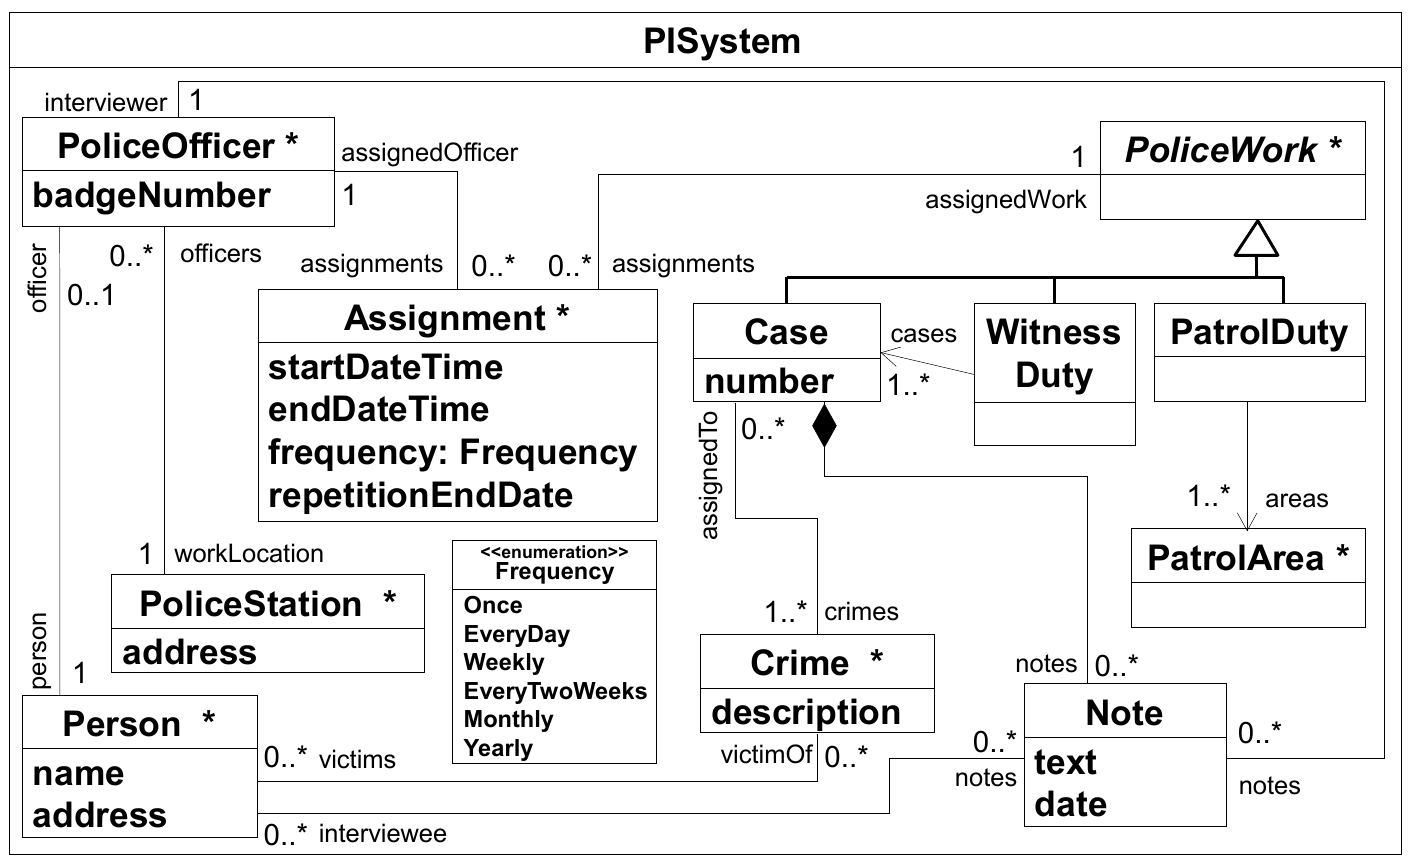
\includegraphics[width=0.6\textwidth]{images/PISystem.png}
\end{tabular} \medskip

\noindent Level 6: Resource response with Quiz: \medskip

\begin{tabular}{|p{0.9\linewidth}}
Complete the containment tree for the following model.

\\
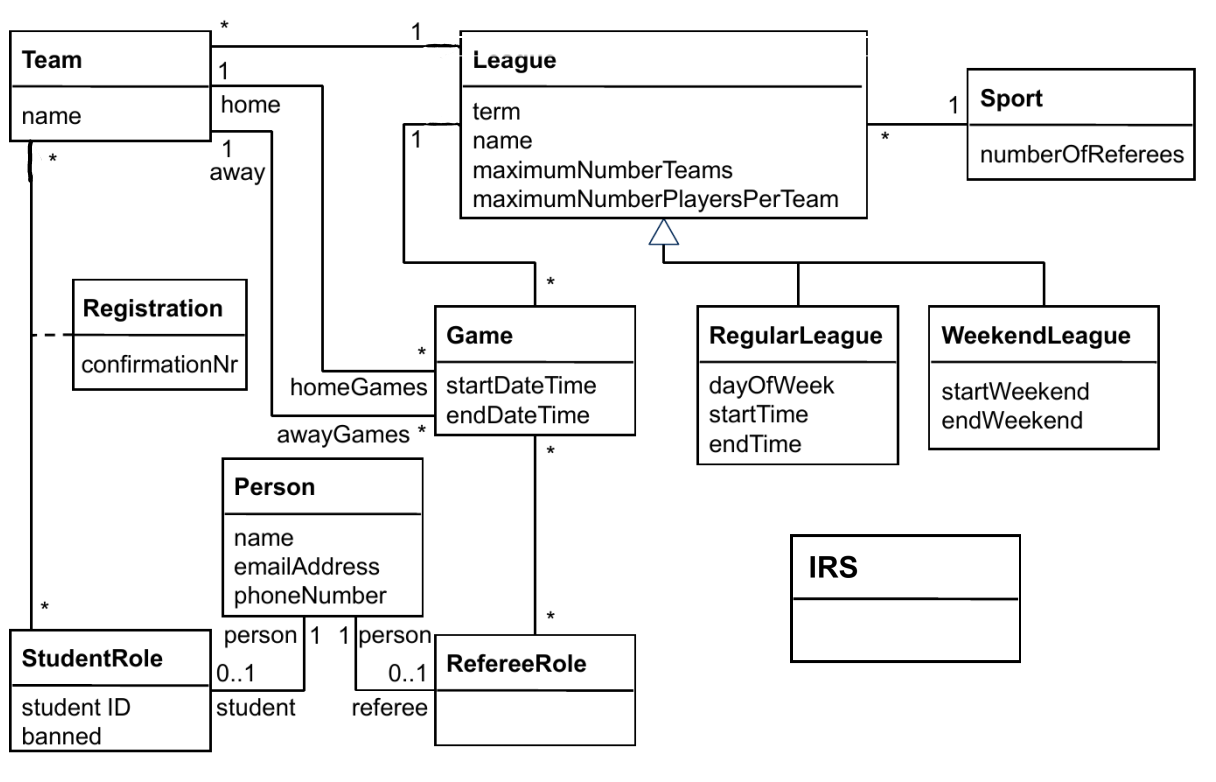
\includegraphics[width=0.6\textwidth]{images/IRS.png}
\end{tabular} \medskip


\subsubsection{Incomplete containment tree}

\noindent Level 1: Highlight solution \medskip

\noindent Level 2: Text response: \medskip

\begin{tabular}{|p{0.9\linewidth}}
What is the relationship between these classes?
\end{tabular} \medskip

\noindent Level 3: Parametrized response: \medskip

\begin{tabular}{|p{0.9\linewidth}}
{containedClass} is a part of \verb|${containerClass}|, so how would you model this?
\end{tabular} \medskip

\noindent Level 4: Resource response with Example: \medskip

\begin{tabular}{|p{0.9\linewidth}}
Observe the following domain model. Every single class is contained in the 
root class, `PISystem`, other than the root class itself.

\\
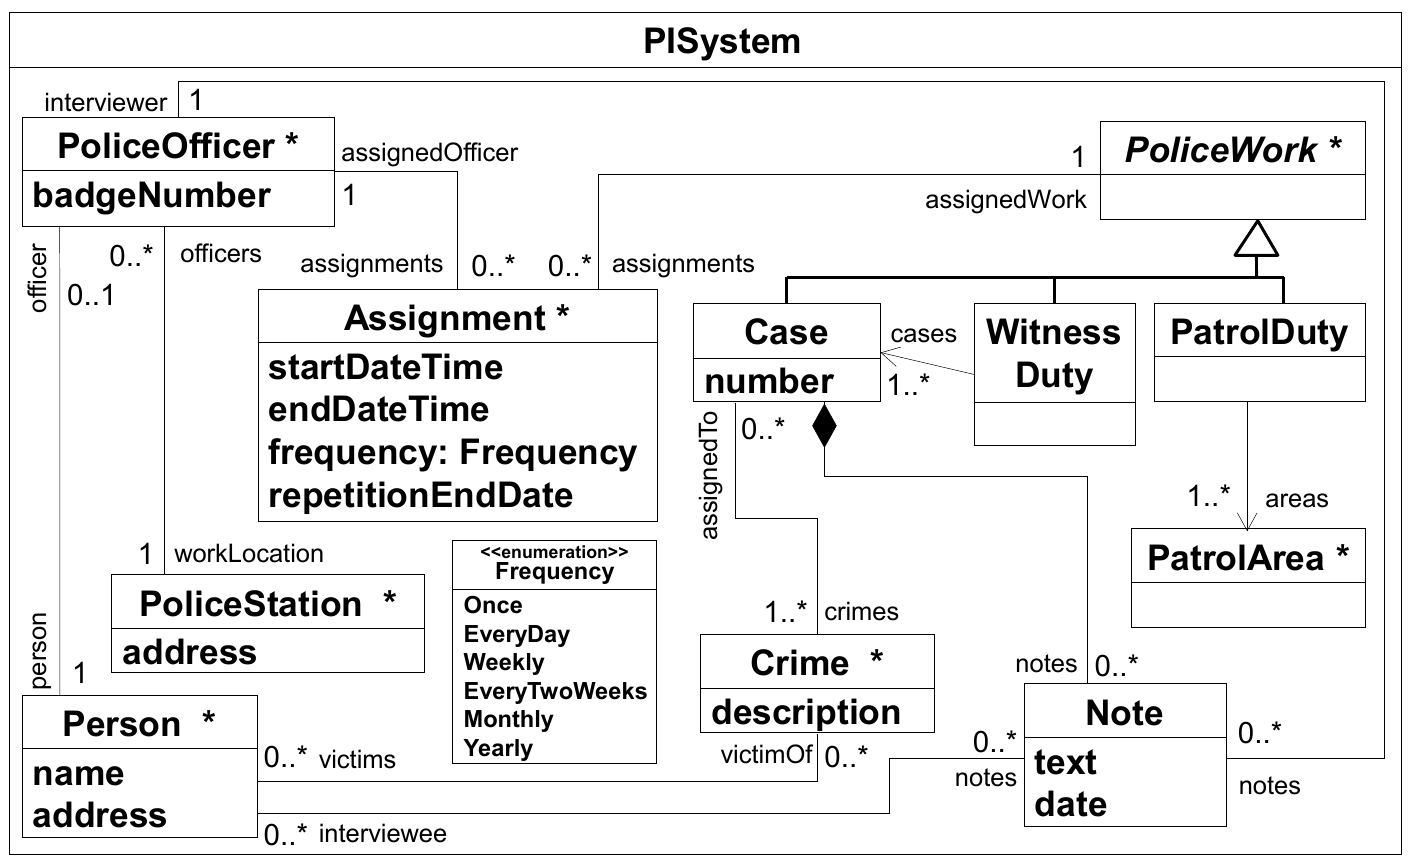
\includegraphics[width=0.6\textwidth]{images/PISystem.png}
\end{tabular} \medskip

\noindent Level 5: Resource response with Quiz: \medskip

\begin{tabular}{|p{0.9\linewidth}}
Complete the containment tree for the following model.

\\
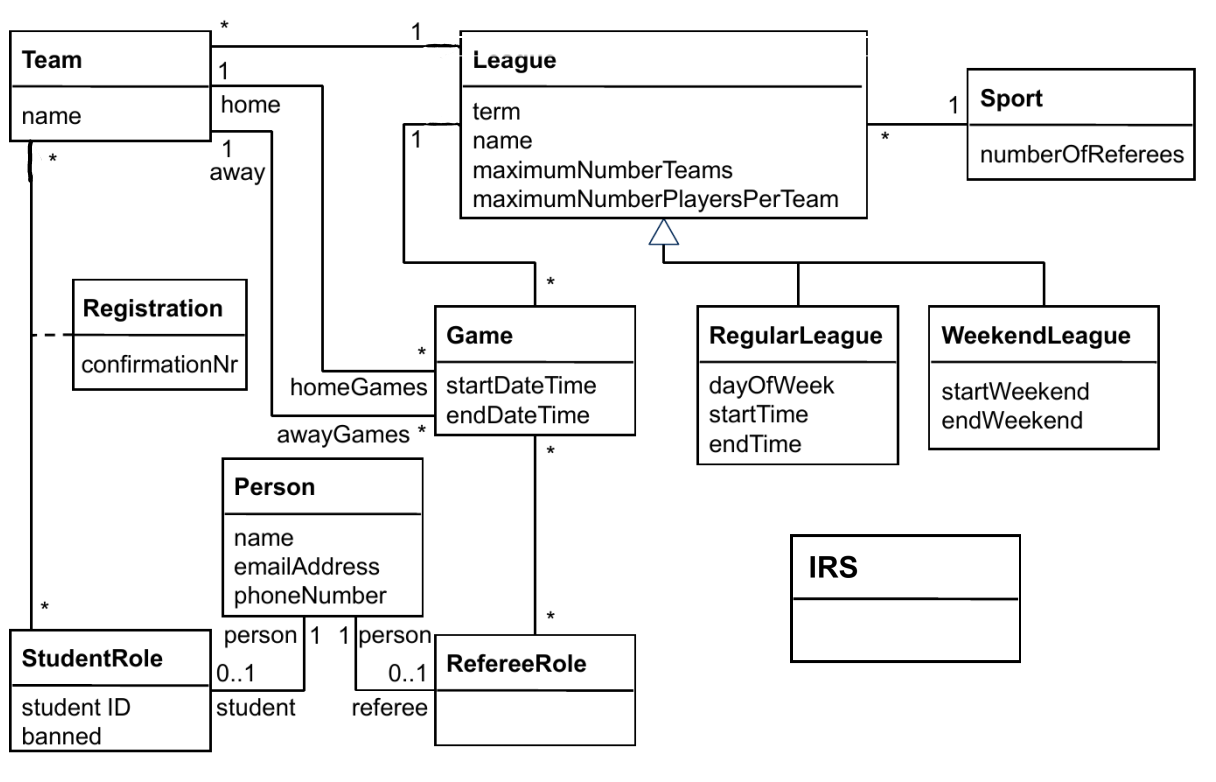
\includegraphics[width=0.6\textwidth]{images/IRS.png}
\end{tabular} \medskip


\subsection{Generalization mistakes}

\subsubsection{Missing generalization}

\noindent Level 1: Highlight solution \medskip

\noindent Level 2: Text response: \medskip

\begin{tabular}{|p{0.9\linewidth}}
What is the relationship between these classes?
\end{tabular} \medskip

\noindent Level 3: Parametrized response: \medskip

\begin{tabular}{|p{0.9\linewidth}}
A \verb|${subclass}| is a \verb|${superclass}|. How should we model this?
\end{tabular} \medskip

\noindent Level 4: Resource response with Quiz: \medskip

\begin{tabular}{|p{0.9\linewidth}}
Place the following classes in an inheritance hierarchy:

\begin{itemize}
    \item Vehicle, LandVehicle, AmphibiousVehicle, AirVehicle, ...
    \item BusVehicle, LuxuryBus, TourBus, BusRoute, ...
\end{itemize}

\end{tabular} \medskip


\subsubsection{Extra generalization}

\noindent Level 1: Highlight solution \medskip

\noindent Level 2: Text response: \medskip

\begin{tabular}{|p{0.9\linewidth}}
Can you find a better way to express this relationship?
\end{tabular} \medskip

Text response: \medskip

\begin{tabular}{|p{0.9\linewidth}}
Is there a [direct ]relationship between these two classes?
\end{tabular} \medskip

\noindent Level 3: Parametrized response: \medskip

\begin{tabular}{|p{0.9\linewidth}}
When creating a generalization between \verb|${wrongSubclass}| and \verb|${wrongSuperclass}|, make sure to follow the \textit{checks for proper generalization}.
\end{tabular} \medskip

\begin{tabular}{|p{0.9\linewidth}}
\verb|${wrongSubclass}| is not a [direct ]subclass of \verb|${wrongSuperclass}|.
\end{tabular} \medskip

\noindent Level 4: Resource response with Quiz: \medskip

\begin{tabular}{|p{0.9\linewidth}}
Place the following classes in an inheritance hierarchy:

\begin{itemize}
    \item Vehicle, LandVehicle, AmphibiousVehicle, AirVehicle, ...
    \item BusVehicle, LuxuryBus, TourBus, BusRoute, ...
\end{itemize}

\end{tabular} \medskip

\noindent Level 5: Resource response with Quiz: \medskip

\begin{tabular}{|p{0.9\linewidth}}
Please review the \textit{checks for proper generalization} lecture material
and complete the following:

The five checks for generalization are:
\begin{itemize}
    \item Obeys the \_\_\_\_\_\_\_\_. (isA rule)
    \item Subclass must retain its \_\_\_\_\_\_\_\_. (distinctiveness)
    \item All \_\_\_\_\_\_\_\_ must make sense in each subclass. (inherited features)
    \item Subclass differs from superclass and other subclasses in \_\_\_\_\_\_\_\_ or \_\_\_\_\_\_\_\_. (behavior, structure)
    \item Subclass must not be \_\_\_\_\_\_\_\_. (instance)
\end{itemize}

\end{tabular} \medskip


\subsubsection{Generalization does not follow isA rule}

\noindent Level 1: Highlight solution \medskip

\noindent Level 2: Text response: \medskip

\begin{tabular}{|p{0.9\linewidth}}
Can you find a better way to express this relationship?
\end{tabular} \medskip

Text response: \medskip

\begin{tabular}{|p{0.9\linewidth}}
Is there a [direct ]relationship between these two classes?
\end{tabular} \medskip

\noindent Level 3: Parametrized response: \medskip

\begin{tabular}{|p{0.9\linewidth}}
When creating a generalization between \verb|${wrongSubclass}| and \verb|${wrongSuperclass}|, make sure to follow the \textit{checks for proper generalization}.
\end{tabular} \medskip

\begin{tabular}{|p{0.9\linewidth}}
\verb|${wrongSubclass}| is not a [direct ]subclass of \verb|${wrongSuperclass}|.
\end{tabular} \medskip

\noindent Level 4: Resource response with Quiz: \medskip

\begin{tabular}{|p{0.9\linewidth}}
Place the following classes in an inheritance hierarchy:

\begin{itemize}
    \item Vehicle, LandVehicle, AmphibiousVehicle, AirVehicle, ...
    \item BusVehicle, LuxuryBus, TourBus, BusRoute, ...
\end{itemize}

\end{tabular} \medskip

\noindent Level 5: Resource response with Quiz: \medskip

\begin{tabular}{|p{0.9\linewidth}}
Please review the \textit{checks for proper generalization} lecture material
and complete the following:

The five checks for generalization are:
\begin{itemize}
    \item Obeys the \_\_\_\_\_\_\_\_. (isA rule)
    \item Subclass must retain its \_\_\_\_\_\_\_\_. (distinctiveness)
    \item All \_\_\_\_\_\_\_\_ must make sense in each subclass. (inherited features)
    \item Subclass differs from superclass and other subclasses in \_\_\_\_\_\_\_\_ or \_\_\_\_\_\_\_\_. (behavior, structure)
    \item Subclass must not be \_\_\_\_\_\_\_\_. (instance)
\end{itemize}

\end{tabular} \medskip


\subsubsection{Subclass not distinct across lifetime}

\noindent Level 1: Highlight solution \medskip

\noindent Level 2: Text response: \medskip

\begin{tabular}{|p{0.9\linewidth}}
Can you find a better way to model this concept?
\end{tabular} \medskip

\noindent Level 3: Parametrized response: \medskip

\begin{tabular}{|p{0.9\linewidth}}
Will a[n] \verb|${nondistinctSubclass}| retain this status over its lifetime?
\end{tabular} \medskip

\noindent Level 4: Resource response with Quiz: \medskip

\begin{tabular}{|p{0.9\linewidth}}
Please review the \textit{checks for proper generalization} lecture material
and complete the following:

The five checks for generalization are:
\begin{itemize}
    \item Obeys the \_\_\_\_\_\_\_\_. (isA rule)
    \item Subclass must retain its \_\_\_\_\_\_\_\_. (distinctiveness)
    \item All \_\_\_\_\_\_\_\_ must make sense in each subclass. (inherited features)
    \item Subclass differs from superclass and other subclasses in \_\_\_\_\_\_\_\_ or \_\_\_\_\_\_\_\_. (behavior, structure)
    \item Subclass must not be \_\_\_\_\_\_\_\_. (instance)
\end{itemize}

\end{tabular} \medskip


\subsubsection{Inherited feature does not make sense for subclass}

\noindent Level 1: Highlight solution \medskip

\noindent Level 2: Text response: \medskip

\begin{tabular}{|p{0.9\linewidth}}
Does this belong here?
\end{tabular} \medskip

\noindent Level 3: Parametrized response: \medskip

\begin{tabular}{|p{0.9\linewidth}}
The \verb|${featureName}| feature of the \verb|${superclass}| class does not make sense for its \verb|${subclass}| subclass.
\end{tabular} \medskip

\noindent Level 4: Resource response with Quiz: \medskip

\begin{tabular}{|p{0.9\linewidth}}
Please review the \textit{checks for proper generalization} lecture material
and complete the following:

The five checks for generalization are:
\begin{itemize}
    \item Obeys the \_\_\_\_\_\_\_\_. (isA rule)
    \item Subclass must retain its \_\_\_\_\_\_\_\_. (distinctiveness)
    \item All \_\_\_\_\_\_\_\_ must make sense in each subclass. (inherited features)
    \item Subclass differs from superclass and other subclasses in \_\_\_\_\_\_\_\_ or \_\_\_\_\_\_\_\_. (behavior, structure)
    \item Subclass must not be \_\_\_\_\_\_\_\_. (instance)
\end{itemize}

\end{tabular} \medskip


\subsubsection{Subclass is an instance of superclass}

\noindent Level 1: Highlight solution \medskip

\noindent Level 2: Text response: \medskip

\begin{tabular}{|p{0.9\linewidth}}
Can you find a better way to express this relationship?
\end{tabular} \medskip

\noindent Level 3: Text response: \medskip

\begin{tabular}{|p{0.9\linewidth}}
Remember the definition of the **isA rule**.[ Instances should not be modeled as subclasses].
\end{tabular} \medskip

\noindent Level 4: Resource response with Example: \medskip

\begin{tabular}{|p{0.9\linewidth}}
A CheckingAccount isA Account, but account1234 is **not** an Account according to the isA Rule.
\end{tabular} \medskip

\noindent Level 5: Resource response with Quiz: \medskip

\begin{tabular}{|p{0.9\linewidth}}
Please review the \textit{checks for proper generalization} lecture material
and complete the following:

The five checks for generalization are:
\begin{itemize}
    \item Obeys the \_\_\_\_\_\_\_\_. (isA rule)
    \item Subclass must retain its \_\_\_\_\_\_\_\_. (distinctiveness)
    \item All \_\_\_\_\_\_\_\_ must make sense in each subclass. (inherited features)
    \item Subclass differs from superclass and other subclasses in \_\_\_\_\_\_\_\_ or \_\_\_\_\_\_\_\_. (behavior, structure)
    \item Subclass must not be \_\_\_\_\_\_\_\_. (instance)
\end{itemize}

\end{tabular} \medskip


\subsubsection{Non-differentiated subclass}

\noindent Level 1: Highlight solution \medskip

\noindent Level 2: Text response: \medskip

\begin{tabular}{|p{0.9\linewidth}}
Is it really necessary to model this as a subclass?
\end{tabular} \medskip

\noindent Level 3: Parametrized response: \medskip

\begin{tabular}{|p{0.9\linewidth}}
\verb|${wrongSubclass}| does not differ from \verb|${wrongSuperclass}| in terms of behavior or structure.
\end{tabular} \medskip

\noindent Level 4: Resource response with Quiz: \medskip

\begin{tabular}{|p{0.9\linewidth}}
Which classes do not belong?
\begin{itemize}
    \item Account, SavingsAccount, OverdrawnAccount, CheckingAccount, MortgageAccount, ClosedAccount
\end{itemize}

\end{tabular} \medskip


\subsubsection{Wrong generalization direction}

\noindent Level 1: Highlight solution \medskip

\noindent Level 2: Text response: \medskip

\begin{tabular}{|p{0.9\linewidth}}
Can you double check this relationship?
\end{tabular} \medskip

\noindent Level 3: Parametrized response: \medskip

\begin{tabular}{|p{0.9\linewidth}}
Is \verb|${superclass}| really a \verb|${subclass}|?[ It should be the other way around.]
\end{tabular} \medskip

\noindent Level 4: Resource response with Quiz: \medskip

\begin{tabular}{|p{0.9\linewidth}}
Place the following classes in an inheritance hierarchy:

\begin{itemize}
    \item Vehicle, LandVehicle, AmphibiousVehicle, AirVehicle, ...
    \item BusVehicle, LuxuryBus, TourBus, BusRoute, ...
\end{itemize}

\end{tabular} \medskip

\noindent Level 5: Resource response with Quiz: \medskip

\begin{tabular}{|p{0.9\linewidth}}
Please review the \textit{checks for proper generalization} lecture material
and complete the following:

The five checks for generalization are:
\begin{itemize}
    \item Obeys the \_\_\_\_\_\_\_\_. (isA rule)
    \item Subclass must retain its \_\_\_\_\_\_\_\_. (distinctiveness)
    \item All \_\_\_\_\_\_\_\_ must make sense in each subclass. (inherited features)
    \item Subclass differs from superclass and other subclasses in \_\_\_\_\_\_\_\_ or \_\_\_\_\_\_\_\_. (behavior, structure)
    \item Subclass must not be \_\_\_\_\_\_\_\_. (instance)
\end{itemize}

\end{tabular} \medskip


\subsubsection{Wrong superclass}

\noindent Level 1: Highlight solution \medskip

\noindent Level 2: Text response: \medskip

\begin{tabular}{|p{0.9\linewidth}}
Can you double check this relationship?
\end{tabular} \medskip

\noindent Level 3: Parametrized response: \medskip

\begin{tabular}{|p{0.9\linewidth}}
Can you (find$|$create) a (better$|$different) superclass for \verb|${subclass}|?[ Look at the problem description closely].
\end{tabular} \medskip

\noindent Level 4: Highlight problem \medskip

\noindent Level 5: Parametrized response: \medskip

\begin{tabular}{|p{0.9\linewidth}}
What is the inheritance hierarchy between \verb|${hierarchy.classes}|?
\end{tabular} \medskip

\noindent Level 6: Resource response with Quiz: \medskip

\begin{tabular}{|p{0.9\linewidth}}
Place the following classes in an inheritance hierarchy:

\begin{itemize}
    \item Vehicle, LandVehicle, AmphibiousVehicle, AirVehicle, ...
    \item BusVehicle, LuxuryBus, TourBus, BusRoute, ...
\end{itemize}

\end{tabular} \medskip




\section{Design pattern mistakes}

\subsection{Player-Role Pattern mistakes}

\subsubsection{Using different Player-Role pattern}

\noindent \textbf{Subclass should be full Player-Role pattern} \medskip


\noindent \textbf{Subclass should be association Player-Role pattern} \medskip


\noindent \textbf{Subclass should be enumeration Player-Role pattern} \medskip


\noindent \textbf{Association should be full Player-Role pattern} \medskip


\noindent \textbf{Association should be subclass Player-Role pattern} \medskip


\noindent \textbf{Association should be enumeration Player-Role pattern} \medskip


\noindent \textbf{Enumeration should be full Player-Role pattern} \medskip


\noindent \textbf{Enumeration should be subclass Player-Role pattern} \medskip


\noindent \textbf{Enumeration should be association Player-Role pattern} \medskip


\noindent \textbf{Full Player-Role pattern should be subclass} \medskip


\noindent \textbf{Full Player-Role pattern should be association} \medskip


\noindent \textbf{Full Player-Role pattern should be enumeration} \medskip


\subsubsection{Missing Player-Role pattern}

\noindent Level 1: Highlight solution \medskip

\noindent Level 2: Text response: \medskip

\begin{tabular}{|p{0.9\linewidth}}
Think carefully about how to model the relationships between these concepts.
\end{tabular} \medskip

\noindent Level 3: Parametrized response: \medskip

\begin{tabular}{|p{0.9\linewidth}}
Modeling all the concepts in one \verb|${playerClass}| class will make it very complicated! Think about adding one or more classes to better represent the domain.
\end{tabular} \medskip

\begin{tabular}{|p{0.9\linewidth}}
[Nice try, but ]a \verb|${firstSubclass}| can also play the role of a \verb|${secondSubclass}|.
\end{tabular} \medskip

\noindent Level 4: Resource response with Reference: \medskip

\begin{tabular}{|p{0.9\linewidth}}
The Player-Role Pattern can be used to capture the fact that an object may play different roles
in different contexts.

\\
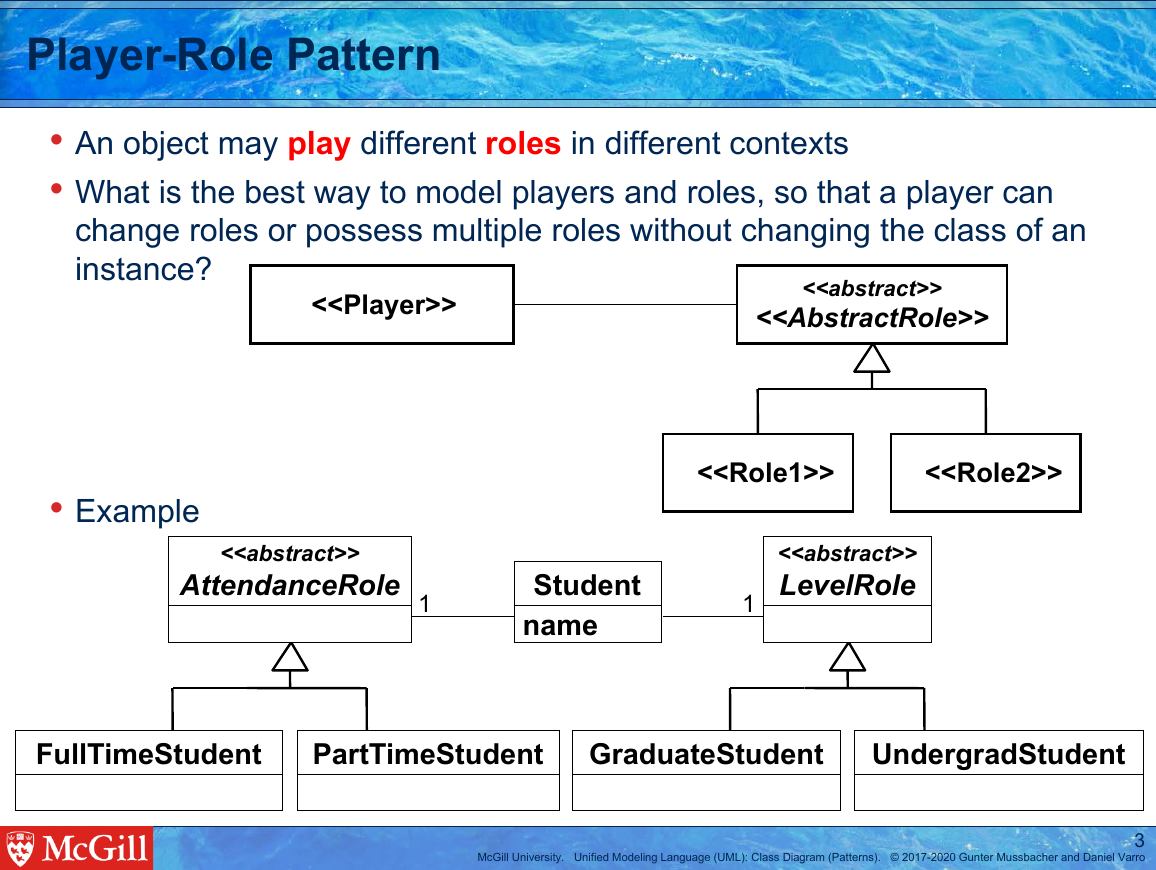
\includegraphics[width=0.6\textwidth]{images/player_role.png}
\end{tabular} \medskip

\noindent Level 5: Resource response with Quiz: \medskip


\begin{tabular}{lcccc}
\hline
\textbf{Solution} &
  \textbf{\begin{tabular}[c]{@{}c@{}}Roles\\ have\\ different\\ features\end{tabular}} &
  \textbf{\begin{tabular}[c]{@{}c@{}}Only one\\ role at\\ a time\end{tabular}} &
  \textbf{\begin{tabular}[c]{@{}c@{}}Different\\ roles\\ over time\end{tabular}} &
  \textbf{\begin{tabular}[c]{@{}c@{}}More than\\ one role\\ at the\\ same time\end{tabular}} \\ \hline
Enumeration         & $\square$ & $\square$ & $\square$ & $\square$ \\
Subclasses          & $\square$ & $\square$ & $\square$ & $\square$ \\
Associations        & $\square$ & $\square$ & $\square$ & $\square$ \\
Player-Role Pattern & $\square$ & $\square$ & $\square$ & $\square$ \\ \hline
\end{tabular}

\subsubsection{Incomplete Player-Role pattern}

\noindent Level 1: Highlight solution \medskip

\noindent Level 2: Text response: \medskip

\begin{tabular}{|p{0.9\linewidth}}
Think carefully about how to model the relationships between these concepts.
\end{tabular} \medskip

\noindent Level 3: Parametrized response: \medskip

\begin{tabular}{|p{0.9\linewidth}}
Modeling all the concepts in one \verb|${playerClass}| class will make it very complicated! Think about adding one or more classes to better represent the domain.
\end{tabular} \medskip

\begin{tabular}{|p{0.9\linewidth}}
[Nice try, but ]a \verb|${firstSubclass}| can also play the role of a \verb|${secondSubclass}|.
\end{tabular} \medskip

\noindent Level 4: Resource response with Reference: \medskip

\begin{tabular}{|p{0.9\linewidth}}
The Player-Role Pattern can be used to capture the fact that an object may play different roles
in different contexts.

\\
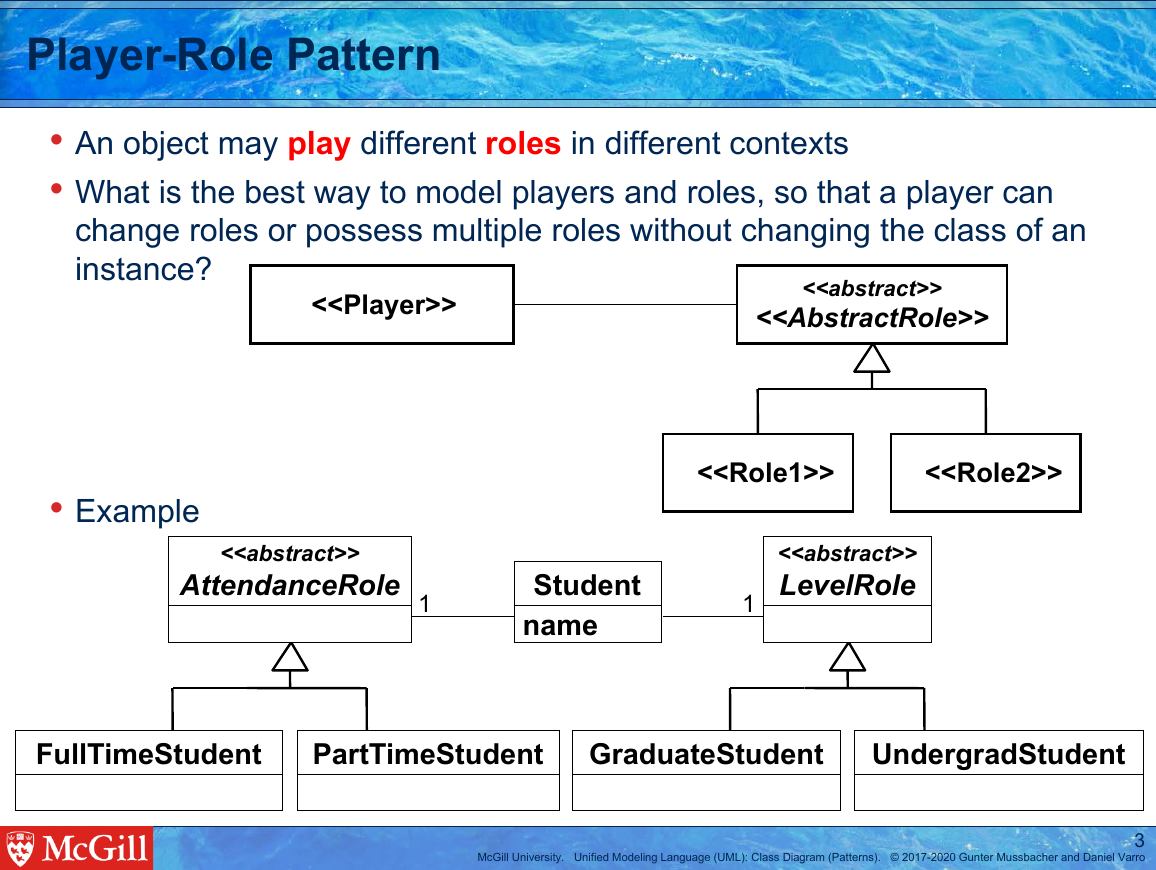
\includegraphics[width=0.6\textwidth]{images/player_role.png}
\end{tabular} \medskip

\noindent Level 5: Resource response with Quiz: \medskip


\begin{tabular}{lcccc}
\hline
\textbf{Solution} &
  \textbf{\begin{tabular}[c]{@{}c@{}}Roles\\ have\\ different\\ features\end{tabular}} &
  \textbf{\begin{tabular}[c]{@{}c@{}}Only one\\ role at\\ a time\end{tabular}} &
  \textbf{\begin{tabular}[c]{@{}c@{}}Different\\ roles\\ over time\end{tabular}} &
  \textbf{\begin{tabular}[c]{@{}c@{}}More than\\ one role\\ at the\\ same time\end{tabular}} \\ \hline
Enumeration         & $\square$ & $\square$ & $\square$ & $\square$ \\
Subclasses          & $\square$ & $\square$ & $\square$ & $\square$ \\
Associations        & $\square$ & $\square$ & $\square$ & $\square$ \\
Player-Role Pattern & $\square$ & $\square$ & $\square$ & $\square$ \\ \hline
\end{tabular}

\subsection{Abstraction-Occurrence pattern mistakes}

\subsubsection{Missing Abstraction-Occurrence pattern}

\noindent Level 1: Highlight solution \medskip

\noindent Level 2: Text response: \medskip

\begin{tabular}{|p{0.9\linewidth}}
Think carefully about how to model the relationships between these concepts.
\end{tabular} \medskip

\noindent Level 3: Parametrized response: \medskip

\begin{tabular}{|p{0.9\linewidth}}
Is there a way to remove the duplicate \verb|${duplicateAttribute}| attribute between \verb|${class1}| and \verb|${class2}|?
\end{tabular} \medskip

\begin{tabular}{|p{0.9\linewidth}}
\verb|${wronglySubclass}| should not be a subclass of \verb|${superclass}|. Is there a design pattern that can be used here?
\end{tabular} \medskip

\begin{tabular}{|p{0.9\linewidth}}
The \verb|${commonAttribute}| is common information for all instances of \verb|${className}|, but this is not enforced.
\end{tabular} \medskip

\noindent Level 4: Resource response with Reference: \medskip

\begin{tabular}{|p{0.9\linewidth}}
The \textit{Abstraction-Occurrence Pattern} can be used to 
represent a set of related objects that share common information but also differ
from each other in an important way.

\\
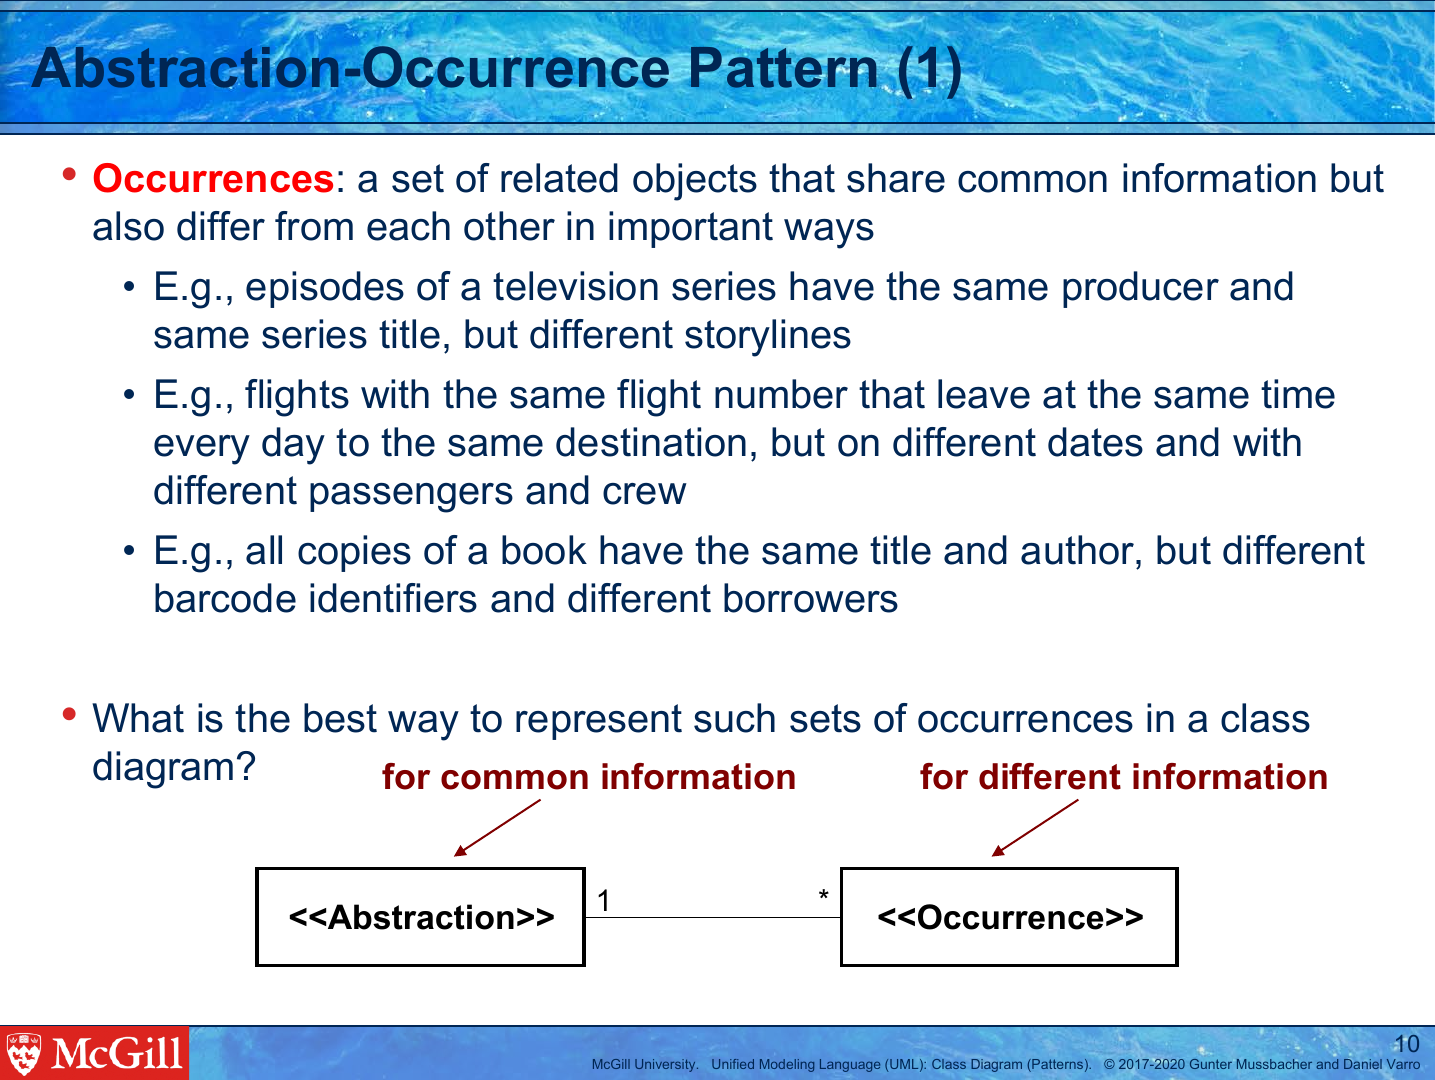
\includegraphics[width=0.6\textwidth]{images/abstraction_occurrence.png}
\end{tabular} \medskip


\subsubsection{Incomplete Abstraction-Occurrence pattern}

\noindent Level 1: Highlight solution \medskip

\noindent Level 2: Text response: \medskip

\begin{tabular}{|p{0.9\linewidth}}
Think carefully about how to model the relationships between these concepts.
\end{tabular} \medskip

\noindent Level 3: Parametrized response: \medskip

\begin{tabular}{|p{0.9\linewidth}}
Is there a way to remove the duplicate \verb|${duplicateAttribute}| attribute between \verb|${class1}| and \verb|${class2}|?
\end{tabular} \medskip

\begin{tabular}{|p{0.9\linewidth}}
\verb|${wronglySubclass}| should not be a subclass of \verb|${superclass}|. Is there a design pattern that can be used here?
\end{tabular} \medskip

\begin{tabular}{|p{0.9\linewidth}}
The \verb|${commonAttribute}| is common information for all instances of \verb|${className}|, but this is not enforced.
\end{tabular} \medskip

\noindent Level 4: Resource response with Reference: \medskip

\begin{tabular}{|p{0.9\linewidth}}
The \textit{Abstraction-Occurrence Pattern} can be used to 
represent a set of related objects that share common information but also differ
from each other in an important way.

\\
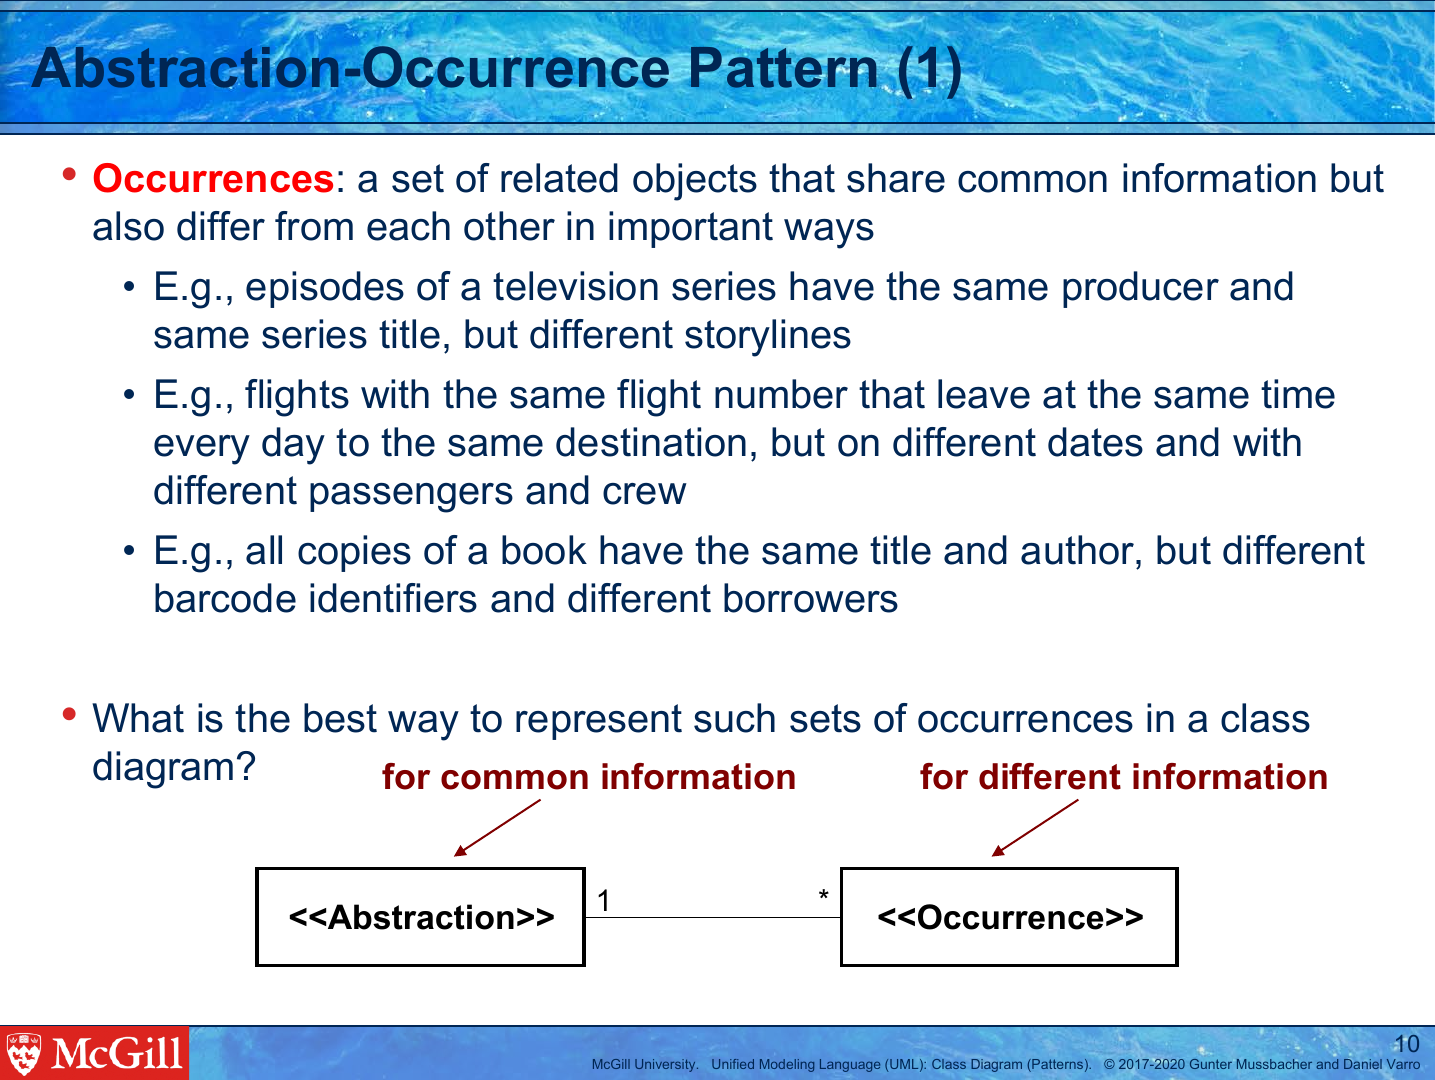
\includegraphics[width=0.6\textwidth]{images/abstraction_occurrence.png}
\end{tabular} \medskip



